\documentclass[11pt]{article}
\usepackage{geometry} 
\usepackage{hyperref}
\usepackage[leftcaption]{sidecap}
\sidecaptionvpos{figure}{c} %position side caption
\usepackage{lineno}
\usepackage{lipsum}
\usepackage{color}
\usepackage{multirow}
\usepackage{booktabs}
\usepackage[pdftex]{graphicx}  
%\usepackage{caption}
\usepackage{natbib}
\usepackage{authblk}
\usepackage[table]{xcolor} %for table line color alteration
\usepackage{subscript}
\renewcommand{\baselinestretch}{1.5}
\bibliographystyle{AJB}

\newcommand{\jri}[1]{\textcolor{blue}{ \emph{\scriptsize  #1}} }
\newcommand{\mbh}[1]{\textcolor{red}{ \emph{\scriptsize  #1}} }
\newcommand{\lev}[1]{\textcolor{green}{\emph{\scriptsize #1}} }

%----------------------------------------
%AUTHORS
%----------------------------------------

\makeatletter
\renewcommand{\maketitle}{\bgroup\vspace*{1cm}\setlength{\parindent}{0pt}
\begin{center}
  \textbf{\@title}
  
  \@author
\end{center}\egroup
}
\makeatother

\title{\LARGE{\bf{Natural variation in teosinte at the domestication locus \emph{teosinte branched1} (\emph{tb1})}}\footnotemark}


\author[2]{Laura Vann}
\author[2,3]{Thomas Kono}
\author[2,4]{Tanja Pyh\"aj\"arvi}
\author[2,5,7]{Matthew B. Hufford}
\author[2,6,7]{Jeffrey Ross-Ibarra}
\affil[2]{Department of Plant Sciences, University of California Davis}
\affil[3]{Department of Agronomy and Plant Genetics, University of Minnesota Twin Cities}
\affil[4]{Department of Biology, University of Oulu}
\affil[5]{Department of Ecology, Evolution, and Organismal Biology, Iowa State University}
\affil[6]{Center for Population Biology and Genome Center, University of California Davis}
\affil[7]{Author for Correspondence}
\date{}

\begin{document}

\flushleft{\large{Vann \emph{et al.}: Variation in teosinte at the \emph{tb1} locus}

{\let\newpage\relax\maketitle}

\begin{linenumbers}
	\pagewiselinenumbers
	\renewcommand\linenumberfont{\normalfont\bfseries\small}

\clearpage
\footnotetext{\flushleft{Manuscript received \line(1,0){120};   revision accepted\line(1,0){120}.}
\vspace*{1cm}
\subsection*{Acknowledgements}
Place brief acknowledgments, if desired, as a separate paragraph, using the following style: �The author(s) thank(s)��. For brevity, do not use first names. Include grant acknowledgments here.
}
\clearpage

%TO DO
%check citations in last paragraph for ter1
%reformat for AJB
%preprint somewhere
%finish fixing paragraph that jeff doesn't like
%check map details
%Code for SAS and command line stuff on Git
%Phenotyping and genotyping data on Git (it's on Figshare?) <- http://dx.doi.org/10.6084/m9.figshare.776926


\begin{flushleft}

\parindent=20pt

\subsection*{Abstract}

The \emph{teosinte branched1} (\emph{tb1}) gene, a repressor of lateral organ growth, is a major QTL involved in branching differences between maize and its wild progenitor, teosinte. Previous work has shown that the insertion of a transposable element (\emph{Hopscotch}) upstream of \emph{tb1} enhances the gene's expression, causing much of the reduction in tillering observed in domesticated maize. Observations of the maize \emph{tb1} allele in teosinte individuals, coupled with estimates of an age of insertion of the \emph{Hopscotch} element that predates domestication, led us to investigate its prevalence and potential role in teosinte. Results from genotyping across many natural populations suggest that the \emph{Hopscotch} element is segregating at a higher than expected frequency in a number of populations of two subspecies of teosinte, \emph{Zea mays} ssp. \emph{parviglumis} and \emph{Zea mays} ssp. \emph{mexicana}. Analysis of linkage disequilibrium between the \emph{Hopscotch} element and variation in surrounding regions does not support a hypothesis of recent introgression from maize into teosinte.  Population genetic signatures, however, are consistent with selection on this locus and suggest the \emph{Hopscotch} insertion at \emph{tb1} may play an ecological role in teosinte. Finally, two greenhouse experiments with \emph{Zea mays} ssp. \emph{parviglumis} do not suggest \emph{tb1} controls tillering in natural populations of this subspecies. Our findings suggest that the role of the \emph{Hopscotch} in tillering in teosinte differs from domesticated maize, and that other loci may play a role in observed variation in this trait.  

\clearpage

\begin{centering}
\section*{INTRODUCTION}
\end{centering}


Domesticated crops and their wild progenitors provide an excellent system in which to study adaptation and genomic changes associated with human-mediated selection \citep{Ross-Ibarra2007}. Perhaps the central focus of the study of domestication has been the identification of genetic variation underlying agronomically important traits such as fruit size and plant architecture \citep{OlsenGross2010}. Additionally, many domesticates show reduced genetic diversity when compared to their wild progenitors, and an understanding of the distribution of diversity in the wild and its phenotypic effects has become increasingly useful to crop improvement \citep{KovachMcCouch2008}. But while some effort has been invested into understanding how wild alleles behave in their domesticated relatives \citep[e.g.][]{Bai2007}, very little is known about the role that alleles found most commonly in domesticates play in natural populations of their wild progenitors \citep{Whitton1997}.

Maize (\emph{Zea mays} ssp. \emph{mays}) was domesticated from the teosinte \emph{Zea mays} ssp. \emph{parviglumis} (hereafter, \emph{parviglumis}) roughly 9,000 B.P. in southwest Mexico \citep{Piperno2009, Matsuoka2002}. Domesticated maize and the teosintes are an attractive system in which to study domestication due to the abundance of genetic tools developed for maize and well-characterized domestication loci \citep{Hufford2012a, Doebley2004, Hufford2012b}. Additionally, large naturally occurring populations of both \emph{Zea mays} ssp. \emph{parviglumis} (the wild progenitor of maize) and \emph{Zea mays} ssp. \emph{mexicana} (highland teosinte; hereafter \emph{mexicana}) can be found throughout Mexico \citep{Wilkes1977, Hufford2013}, and genetic diversity of these taxa is estimated to be high \citep{Ross-Ibarra2009}.

Many morphological changes are associated with maize domestication, and understanding the genetic basis of these changes has been a focus of maize research for a number of years \citep{Doebley2004}. One of the most dramatic changes is found in plant architecture: domesticated maize is characterized by a central stalk with few tillers and lateral branches terminating in a female inflorescence, while teosinte is highly tillered and bears tassels (male inflorescences) at the end of its lateral branches. The \emph{teosinte branched1} (\emph{tb1}) gene, a repressor of organ growth, was identified as a major QTL involved in  branching \citep{DoebleyStecGustus1995} and tillering \citep{DoebleyStec1991} differences between maize and teosinte.  A 4.9 kb retrotransposon (\emph{Hopscotch}) insertion into the upstream control region of \emph{tb1} in maize acts to enhance expression of \emph{tb1}, thus repressing lateral organ growth \citep{Doebley1997, Studer2011}.  Dating of the \emph{Hopscotch} retrotransposon suggests that its insertion predates the domestication of maize, leading to the hypothesis that it was segregating as standing variation in ancient populations of teosinte and increased to high frequency in maize due to selection during domestication \citep{Studer2011}. The effects of the \emph{Hopscotch} insertion have been studied in maize \citep{Studer2011}, and analysis of teosinte alleles at \emph{tb1} has identified functionally distinct allelic classes \citep{StuderDoebley2012}, but little is known about the role of \emph{tb1} or the \emph{Hopscotch} insertion in natural populations of teosinte.

In teosinte and other plants that grow at high population density, individuals detect competition from neighbors via the ratio of red to far-red light.  An increase in far-red relative to red light accompanies shading and triggers the shade avoidance syndrome: a suite of physiological and morphological changes such as reduced tillering, increased plant height and early flowering \citep{KebromBrutnell2007}. The \emph{tb1} locus appears to play an important role in the shade avoidance pathway in \emph{Zea mays} and other grasses and may therefore be crucial to the ecology of teosinte \citep{KebromBrutnell2007, LukensDoebley1999}.  In this study we aim to characterize the distribution of the \emph{Hopscotch} insertion in \emph{parviglumis}, \emph{mexicana}, and landrace maize, and to examine the phenotypic effects of the insertion in \emph{parviglumis}. We use a combination of PCR genotyping for the \emph{Hopscotch} element in our full panel and sequencing of two small regions upstream of \emph{tb1} in a subset of teosinte populations to explore patterns of genetic variation at this locus. Finally, we test for an association between the \emph{Hopscotch} element and tillering phenotypes in a population of \emph{parviglumis}.

\begin{centering}
\section*{MATERIALS AND METHODS}
\end{centering}

\subsection*{Sampling and genotyping}

We sampled 1,110 individuals from 350 accessions (247 maize landraces, 17 \emph{mexicana} populations, and 86 \emph{parviglumis} populations) and assessed the presence or absence of the \emph{Hopscotch} insertion (Table~S1 and Table~S2). DNA was extracted from leaf tissue using a modified CTAB approach \citep{DoyleDoyle1990, Maloof1984}. We designed primers using PRIMER3 \citep{RozenSkaletsky2000} implemented in Geneious \citep{Kearse2012} to amplify the entire \emph{Hopscotch} element, as well as an internal primer allowing us to simultaneously check for possible PCR bias between presence and absence of the \emph{Hopscotch} insertion. Two PCRs were performed for each individual, one with primers flanking the \emph{Hopscotch} (HopF/HopR) and one with a flanking primer and an internal primer (HopF/HopIntR). Primer sequences are HopF, {\small 5'-TCGTTGATGCTTTGATGGATGG-3'}; 
HopR, {\small 5'-AACAGTATGATTTCATGGGACCG-3'}; and HopIntR, {\small  5'-CCTCCACCTCTCATGAGATCC-3'} (Fig.~S1, Fig.~S2) \mbh{Primers in Fig.~S1 should be labeled}. Homozygotes show a single band for absence of the element ($\sim$300bp) and two bands for presence of the element ($\sim$5kb and XX \mbh{LV, please add the size of the second band}), whereas heterozygotes are three-banded (Fig.~S2). When only one PCR resolved well, we scored one allele for the individual. We used Phusion High Fidelity Enzyme (Thermo Fisher Scientific Inc., Waltham, Massachusetts, USA) and the following conditions for amplifications: 98$^{\circ}$C for 3 min, 30 cycles of 98$^{\circ}$C for 15 s, 65$^{\circ}$C for 30 s, and 72$^{\circ}$C for 3 min 30 s, with a final extension of 72$^{\circ}$C for 10 min. PCR products were visualized on a 1\% agarose gel and scored for presence/absence of the \emph{Hopscotch} based on band size.

\subsection*{Sequencing}

In addition to genotyping, we chose a subset of \emph{parviglumis} individuals for sequencing. We chose twelve individuals from each of four populations from Jalisco state, Mexico (San Lorenzo, La Mesa, Ejutla A, and Ejutla B). For amplification and sequencing, we selected two regions approximately 600bp in size from within the 5' UTR of \emph{tb1} (Region 1) and from 1,235bp upstream of the start of the \emph{Hopscotch} (66,169bp upstream from the start of the \emph{tb1} ORF; Region 2). We designed the following primers using PRIMER3 \citep{RozenSkaletsky2000}: for the 5' UTR, {\small 5-'GGATAATGTGCACCAGGTGT-3'} and {\small 5'-GCGTGCTAGAGACACYTGTTGCT-3'}; for the 66kb upstream region, {\small 5'-TGTCCTCGCCGCAACTC-3'} and {\small 5'-TGTACGCCCGCCCCTCATCA-3'} (Fig.~S1). We used Taq polymerase (New England Biolabs Inc., Ipswich, Massachusetts, USA) and the following thermal cycler conditions to amplify fragments: 94$^{\circ}$C for 3 min, 30 cycles of 92$^{\circ}$C for 40 s, annealing for 1 min, 72$^{\circ}$C for 40 s, and a final 10 min extension at 72$^{\circ}$C. Annealing temperatures for Region 1 and Region 2 were 59.7$^{\circ}$C and 58.8$^{\circ}$C, respectively. To clean excess primer and dNTPs we added two units of Exonuclease1 and 2.5 units of Antarctic Phosphatase to 8.0 $\mu$L of amplification product. This mix was placed on a thermal cycler with the following program: 37$^{\circ}$C for 30 min, 80$^{\circ}$C for 15 min, and a final cool-down step to 4$^{\circ}$C. 

We cloned cleaned fragments into a TOPO-TA vector (Life Technologies, Grand Island, New York, USA) using OneShot TOP10 chemically competent \emph{E. coli} cells, with an extended ligation time of 30 min for a complex target fragment. We plated cells on LB agar plates containing kanamycin, and screened colonies using vector primers M13 Forward and M13 Reverse under the following conditions: 96$^{\circ}$C for 5 min; then 35 cycles at 96$^{\circ}$C for 30 s, 53$^{\circ}$C for 30 s, 72$^{\circ}$C for 2 min; and a final extension at 72$^{\circ}$C for 4 min. We visualized amplification products for incorporation of our insert on a 1\% agarose TAE gel.

Amplification products with successful incorporation of our insert were cleaned using Exonuclease 1 and Antarctic Phosphatase following the procedures detailed above, and sequenced with vector primers M13 Forward and M13 Reverse using Sanger sequencing at the College of Agriculture and Environmental Sciences (CAES) sequencing center at UC Davis. We aligned and trimmed primer sequences from resulting sequences using the software Geneious \citep{Kearse2012}. Following alignment, we verified singleton SNPs by sequencing an additional one to four colonies from each clone. If the singleton was not present in these additional sequences it was considered an amplification or cloning error, and we replaced the base with the base of the additional sequences. If the singleton appeared in at least one of the additional sequences we considered it a real variant and kept it for further analyses. 

\subsection*{Genotyping analysis}

We examined discrepancies between observed and expected genotype frequencies by calculating Hardy-Weinberg Equilibrium (HWE).  To calculate differentiation between populations (F\textsubscript{ST}) and subspecies (F\textsubscript{CT}) we used HierFstat \citep{Goudet2005}. These analyses only included populations in which 8 or more individuals were sampled. To test the hypothesis that the \emph{Hopscotch} insertion may be adaptive under certain environmental conditions, we looked for significant associations between the \emph{Hopscotch} frequency and environmental variables using BayEnv \citep{Coop2010}. BayEnv creates a covariance matrix of relatedness between populations and then tests a null model that allele frequencies in populations are determined by the covariance matrix of relatedness alone against the alternative model that allele frequencies are determined by a combination of the covariance matrix and an environmental variable, producing a posterior probability (\emph{i.e.,} Bayes Factor; \citealt{Coop2010}). We used genotyping and covariance data from \citet{Pyhajarvi2013} for BayEnv, with the \emph{Hopscotch} insertion coded as an additional SNP (Table~S3). Environmental data were obtained from \url{www.worldclim.org}, the Harmonized World Soil Database \citep{FAOHWSD} and \url{www.harvestchoice.org} and summarized by principle component analysis following \citet{Pyhajarvi2013}.

\subsection*{Sequence analysis}

For population genetic analyses of sequenced Region 1 and sequenced Region 2 we used the  Libsequence package \citep{Thornton2003} to calculate pairwise F\textsubscript{ST} between populations and to calculate standard diversity statistics (number of haplotypes, haplotype diversity, Watterson's estimator $\hat\theta_W$, pairwise nucleotide diversity $\hat\theta_\pi$, and Tajima's D). To produce a visual representation of differentiation between sequences and examine patterns in sequence clustering by \emph{Hopscotch} genotype we used Phylip (\url{http://evolution.genetics.washington.edu/phylip.html}), creating neighbor-joining trees with bootstrap-supported nodes (100 repetitions). For creation of trees we also included homologous sequence data from Maize HapMapV2 \citep{Chia2012} for teosinte inbred lines (TILs), some of which are known to be homozygous for the \emph{Hopscotch} insertion (TIL03, TIL17, TIL09), as well as 59 lines of domesticated maize.

\subsection*{Introgression analysis}

In order to assess patterns of linkage disequilibrium (LD) around the \emph{Hopscotch} element in the context of chromosomal patterns of LD we used Tassel \citep{Bradbury2007} and calculated LD between SNPs across chromosome 1 using previously published data from twelve plants each of the Ejutla A (EjuA), Ejutla B (EjuB), San Lorenzo (SLO), and La Mesa (MSA) populations \citep{Pyhajarvi2013}. We chose these populations because we had both genotyping data for the \emph{Hopscotch} as well as chromosome-wide SNP data for chromosome 1. For each population we filtered the initial set of 5,897 SNPs on chromosome 1 to accept only SNPs with a minor allele frequency of at least 0.1, resulting in 1,671, 3,023, 3,122, and 2,167 SNPs for SLO, EjuB, EjuA, and MSA, respectively. We then used Tassel \citep{Bradbury2007} to calculate linkage disequilibrium ($r^{2}$) across chromosome 1 for each population. 

We examined evidence of introgression on chromosome 1 in these same four populations (EjuA, EjuB, MSA, SLO) using STRUCTURE \citep{Falush2003} and phased data from \citet{Pyhajarvi2013}, combined with the corresponding SNP data from a diverse panel of 282 maize lines \citep{Cook2012}. SNPs were anchored in a modified version of the IBM genetic map \citep{Gerke2013}. We created haplotype blocks using a custom Perl script that grouped SNPs separated by less than 5kb into haplotypes. We ran STRUCTURE at K=2 under the linkage model, performing 3 replicates with an MCMC burn-in of 10,000 steps and 50,000 steps post burn-in.

\subsection*{Phenotyping of \emph{parviglumis}}

To investigate the phenotypic effects of the \emph{Hopscotch} insertion in teosinte, we conducted an initial phenotyping trial (Phenotyping 1). We germinated 250 seeds of \emph{parviglumis} collected in Jalisco state, Mexico (population San Lorenzo) \citep{Hufford2010} where the \emph{Hopscotch} is segregating at highest frequency (0.44) in our initial genotyping sample set. In order to maximize the likelihood of finding the \emph{Hopscotch} in our association population we selected seeds from sites where genotyped individuals were homozygous or heterozygous for the insertion. We chose between 10-13 seeds from each of 23 sampling sites. We treated seeds with fungicide and germinated them in petri dishes with filter paper. Following germination, 206 successful germinations were planted into one-gallon pots with potting soil and randomly spaced one foot apart on greenhouse benches. Plants were watered three times a day by hand and with an automatic drip containing 10-20-10 fertilizer. 

Starting on day 15, we measured tillering index as the ratio of the sum of tiller lengths to the height of the plant \citep{Briggs2007}. Following initial measurements, we phenotyped plants for tillering index every 5 days through day 40, and then on day 50 and day 60. On day 65 we measured culm diameter between the third and fourth nodes of each plant. Culm diameter is not believed to be correlated with tillering index or variation at \emph{tb1}. Following phenotyping we extracted DNA from all plants using a modified SDS extraction protocol (\url{http://www.ars.usda.gov}). \jri{what is this url?} We genotyped individuals for the \emph{Hopscotch} insertion following the protocols listed above. Based on these initial data, we conducted a \emph{post hoc} power analysis using data from day 40 of Phenotyping 1, indicating that a minimum of 71 individuals in each genotypic class would be needed to detect the observed effect of the \emph{Hopscotch} on tillering index.

We performed a second phenotyping experiment (Phenotyping 2) in which we germinated 372 seeds of \emph{parviglumis}, choosing equally between sites previously determined to have or not have the \emph{Hopscotch} insertion. Seeds were germinated and planted on day 7 post fruit-case removal into two gallon pots. Plants were watered twice daily, alternating between fertilized and non-fertilized water. We began phenotyping successful germinations (302 plants) for tillering index on day 15 post fruit-case removal, and phenotyped every five days until day 50. At day 50 we measured culm diameter between the third and fourth nodes. We extracted DNA and genotyped plants following the same guidelines as in Phenotyping 1. 

Tillering index data for each genotypic class did not meet the criteria for a repeated measures ANOVA, so we transformed the data using a Box-Cox transformation ($\alpha=0$ \mbh{what is the alpha value here?}; Car Package for R, \citealt{FoxWeisberg2011}) to improve the normality and homogeneity of variance among genotype classes.  We analyzed relationships between genotype and tillering index and tiller number using a repeated measures ANOVA through a general linear model function implemented in SAS v.9.3 (SAS Institute Inc., Cary, NC, USA). Additionally, in order to compare any association between \emph{Hopscotch} genotype and tillering and associations at other presumably unrelated traits, we performed an ANOVA between culm diameter and genotype using the same general linear model in SAS.

\begin{centering}
\section*{RESULTS}
\end{centering}

\subsection*{Genotyping}

Genotype of the \emph{Hopscotch} insertion was confirmed with two PCRs for 837 individuals. Among the 247 maize landrace accessions genotyped, all but eight were homozygous for the presence of the insertion (Table~S1 and Table~S2). Within our \emph{parviglumis} and \emph{mexicana} samples we found the \emph{Hopscotch} insertion segregating in 37 and 4 populations, respectively, and at highest frequency in the states of Jalisco, Colima, and Michoac\'{a}n in central-western Mexico (Fig. \ref{Fig1Map}). 
%We examined Hardy-Weinberg equilibrium in a total of 14 populations (10 \emph{parviglumis} and 4 \emph{mexicana}) with more than 8 individuals sampled per population. Three populations (RIMPA0073, RIMPA0093, and RIMPA0158) show evidence of deviations from expected genotype frequencies under the assumptions of HWE (p$<$0.05). \mbh{Jeff mentioned this needs to be fully reported in a supplementary table; alternatively we can just delete the result since we do not interpret or use it later in the manuscript.}

Using our \emph{Hopscotch} genotyping, we calculated differentiation between populations (F\textsubscript{ST}) and subspecies (F\textsubscript{CT}) for populations in which we sampled 8 or more alleles. We found that F\textsubscript{CT} = 0, and levels of F\textsubscript{ST} among populations within each subspecies (0.22) and among all populations (0.23) \jri{are these an average of pairwise or is this calculated among all pops?} are similar to those reported genome-wide in previous studies (\citealt{Pyhajarvi2013}; Table \ref{Table1Fst}). Although we found large variation in \emph{Hopscotch} allele frequency among our populations, BayEnv analysis did not indicate a correlation between the \emph{Hopscotch} insertion and environmental variables (all Bayes Factors $<$ 1; Table~S3). 

%Figure 1 Map 
%--------------------------------------------
\begin{SCfigure}[][t!]
  \centering \label{Fig1Map}
   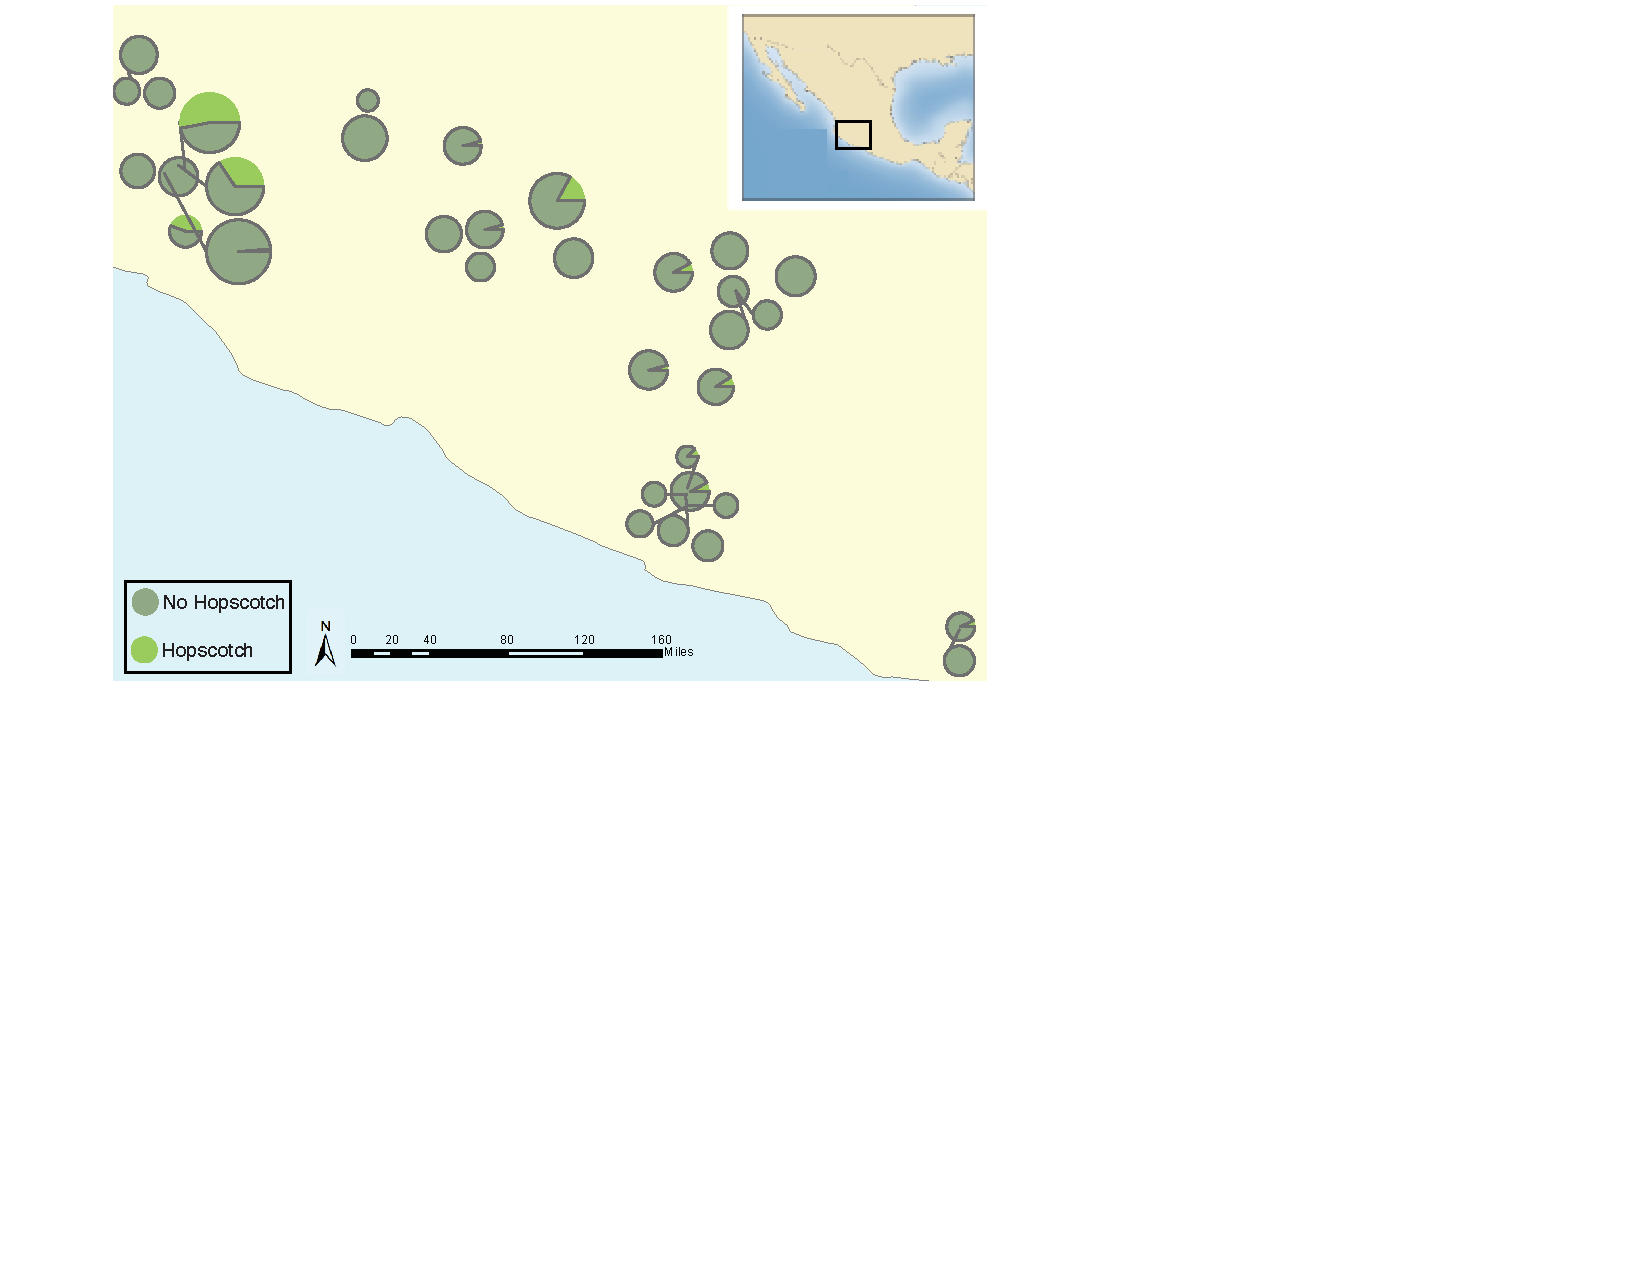
\includegraphics[width=0.7\textwidth]{Fig1Map.pdf}
    \caption{Map showing the frequency of the \emph{Hopscotch} allele in populations of \emph{parviglumis} where we sampled more than 6 individuals. Size of circles reflects number of alleles sampled. } 
\end{SCfigure}
%--------------------------------------------

% Table 1
\begin{table}[htbp]
\rowcolors{2}{gray!25}{white}
  \centering
  \caption{Pairwise F\textsubscript{ST} values from sequence and \emph{Hopscotch} genotyping data}
  
    \begin{tabular}{cccc}\\\toprule
    \textbf{Comparison} & \textbf{Region 1} & \textbf{Region 2} & \textbf{\emph{Hopscotch}} \\\midrule
    EjuA \& EjuB & 0     & 0     & 0 \\
    EjuA \& MSA & 0.326 & 0.328 & 0.186 \\
    EjuA \& SLO & 0.416 & 0.258 & 0.280 \\
    EjuB \& MSA & 0.397 & 0.365 & 0.188 \\
    EjuB \& SLO & 0.512  & 0.290 & 0.280 \\
    MSA \& SLO & 0.007  & 0 & 0.016 \\\bottomrule
    \end{tabular}
  \label{Table1Fst}
\end{table}

\subsection*{Sequencing}

To investigate patterns of sequence diversity and linkage disequilibrium (LD) in the \emph{tb1} region, we sequenced two small ($<$1kb) regions upstream of the \emph{tb1} ORF in four populations. After alignment and singleton checking we recovered 48 and 40 segregating sites for the 5' UTR region (Region 1) and the 66kb upstream region (Region 2), respectively. For Region 1, Ejutla A has the highest values of haplotype diversity, and $\theta_\pi$, while Ejutla B and La Mesa have comparable values of these summary statistics, and San Lorenzo has much lower values. Additionally, Tajima's D is strongly negative in the two Ejutla populations and La Mesa, but is less negative in San Lorenzo (Table \ref{Table2Diversity}). \mbh{need to reference \emph{Hopscotch} frequencies in supplemental table somewhere} For Region 2, haplotype diversity and $\theta_\pi$, are similar for Ejutla A and Ejutla B, while La Mesa and San Lorenzo have slightly lower values for these statistics (Table \ref{Table2Diversity}). Tajima's D is positive in all populations except San Lorenzo, \mbh{is the table wrong? MSA is the only negative value in the table} indicating an excess of low frequency variants in this population (Table \ref{Table2Diversity}). Pairwise values of F\textsubscript{ST} within population pairs Ejutla A/Ejutla B and San Lorenzo/La Mesa are 0 for both sequenced regions as well as for the \emph{Hopscotch} \jri{table 1 shows 0.016 for hopscotch, not 0. which is right?}, while they are high for other population pairs (Table \ref{Table1Fst}). Neighbor joining trees of our sequence data and data from the teosinte inbred lines (TILs; data from Maize HapMapV2, \citealt{Chia2012}) do not reveal any clear clustering pattern with respect to population or \emph{Hopscotch} genotype (Figure~S3); individuals within our sample that have the \emph{Hopscotch} insertion do not group with the teosinte inbred lines or domesticated maize that have the \emph{Hopscotch} insertion. 

% Table 2 Diversity Statistics
\begin{table}[htbp]
\rowcolors{2}{gray!25}{white}
  \centering
  \caption{Population genetic statistics from resequenced regions near the \emph{tb1} locus}
    \begin{tabular}{ccccc}\\\toprule
    \textbf{Population} & \# \textbf{Haplotypes} & \textbf{Hap. Diversity} & \textbf{$\hat\theta_\pi$}    & \textbf{Tajima's D} \\\midrule
    \multicolumn{5}{c}{\textit{Region 1(5' UTR)}} \\
    \multicolumn{1}{c}{EJUA} & 8     & 0.859 & 0.005 & -1.650 \\
    \multicolumn{1}{c}{EJUB} & 5     & 0.709 & 0.004 & -1.831 \\
    \multicolumn{1}{c}{MSA} & 6     & 0.682 & 0.004 & -1.755 \\
    \multicolumn{1}{c}{SLO} & 3     & 0.318 & 0.001 & -0.729 \\
    \multicolumn{5}{c}{\textit{Region 2 (66kb upstream)}} \\
    \multicolumn{1}{c}{EJUA} & 8     & 0.894 & 0.018 & 0.623 \\
    \multicolumn{1}{c}{EJUB} & 8     & 0.894 & 0.016 & 0.295 \\
    \multicolumn{1}{c}{MSA} & 3     & 0.682 & 0.011 & -0.222 \\
    \multicolumn{1}{c}{SLO} & 4     & 0.742 & 0.014 & 0.932 \\\bottomrule
    \end{tabular}
  \label{Table2Diversity}
\end{table}

\subsection*{Evidence of introgression} %JRI HERE

The highest frequency of the \emph{Hopscotch} insertion in teosinte was found in \emph{parviglumis} sympatric with cultivated maize. Our initial hypothesis was that the high frequency of the \emph{Hopscotch} element in these populations could be attributed to introgression from maize into teosinte. To investigate this possibility we examined overall patterns of linkage disequilibrium across chromosome one and specifically in the \emph{tb1} region. If the \emph{Hopscotch} is found in these populations due to recent introgression we would expect to find large blocks of linked markers near this element. We find no evidence of elevated linkage disequilibrium between the \emph{Hopscotch} and SNPs surrounding the \emph{tb1} region in our resequenced populations (Fig. \ref{Fig2LD}), and $r^{2}$ in the \emph{tb1} region  does not differ significantly between populations with (average $r^{2}$ of 0.085) and without (average $r^{2}=0.082$) the \emph{Hopscotch} genotype. In fact, average $r^{2}$ is lower in the \emph{tb1} region ($r^{2}=0.056$) than across the rest of chromosome 1 ($r^{2}=0.083$) (\ref{Table3R2}). \mbh{LV, please go through and make sure the data entered into all the tables is correct.  In Table3, both sequenced regions were labeled as "Region 1".  I changed the second to Region 2 but don't know if the data in this column are really from Region 2}

% Table 3 $r^{2}$ values
\begin{table}[htbp]
\rowcolors{2}{gray!25}{white}
  \centering
  \caption{$r^{2}$ values between SNPs on chromosome 1, in the broad \emph{tb1} region, within the 5' UTR of \emph{tb1} (Region 1), and 66kb upstream of \emph{tb1} (Region 2).}
    \begin{tabular}{ccccc}\\\toprule
    \textbf{Population} & \textbf{Chr. 1} & \textbf{\emph{tb1} region} & \textbf{Region 1} & \textbf{Region 2} \\\midrule
    Ejutla A & 0.095 & 0.050 & 0.747 & 0.215 \\
    Ejutla B & 0.069 & 0.051 & 0.660 & 0.186 \\
    La Mesa & 0.070 & 0.053 & 0.914 & 0.766 \\
    San Lorenzo & 0.101 & 0.067 & 0.912 & 0.636 \\
    \bottomrule
    \end{tabular}
  \label{Table3R2}
\end{table}

% Figure 2. LD plots
%-------------------------------------------------------------------
\begin{figure*}[!t]
  \begin{center}
   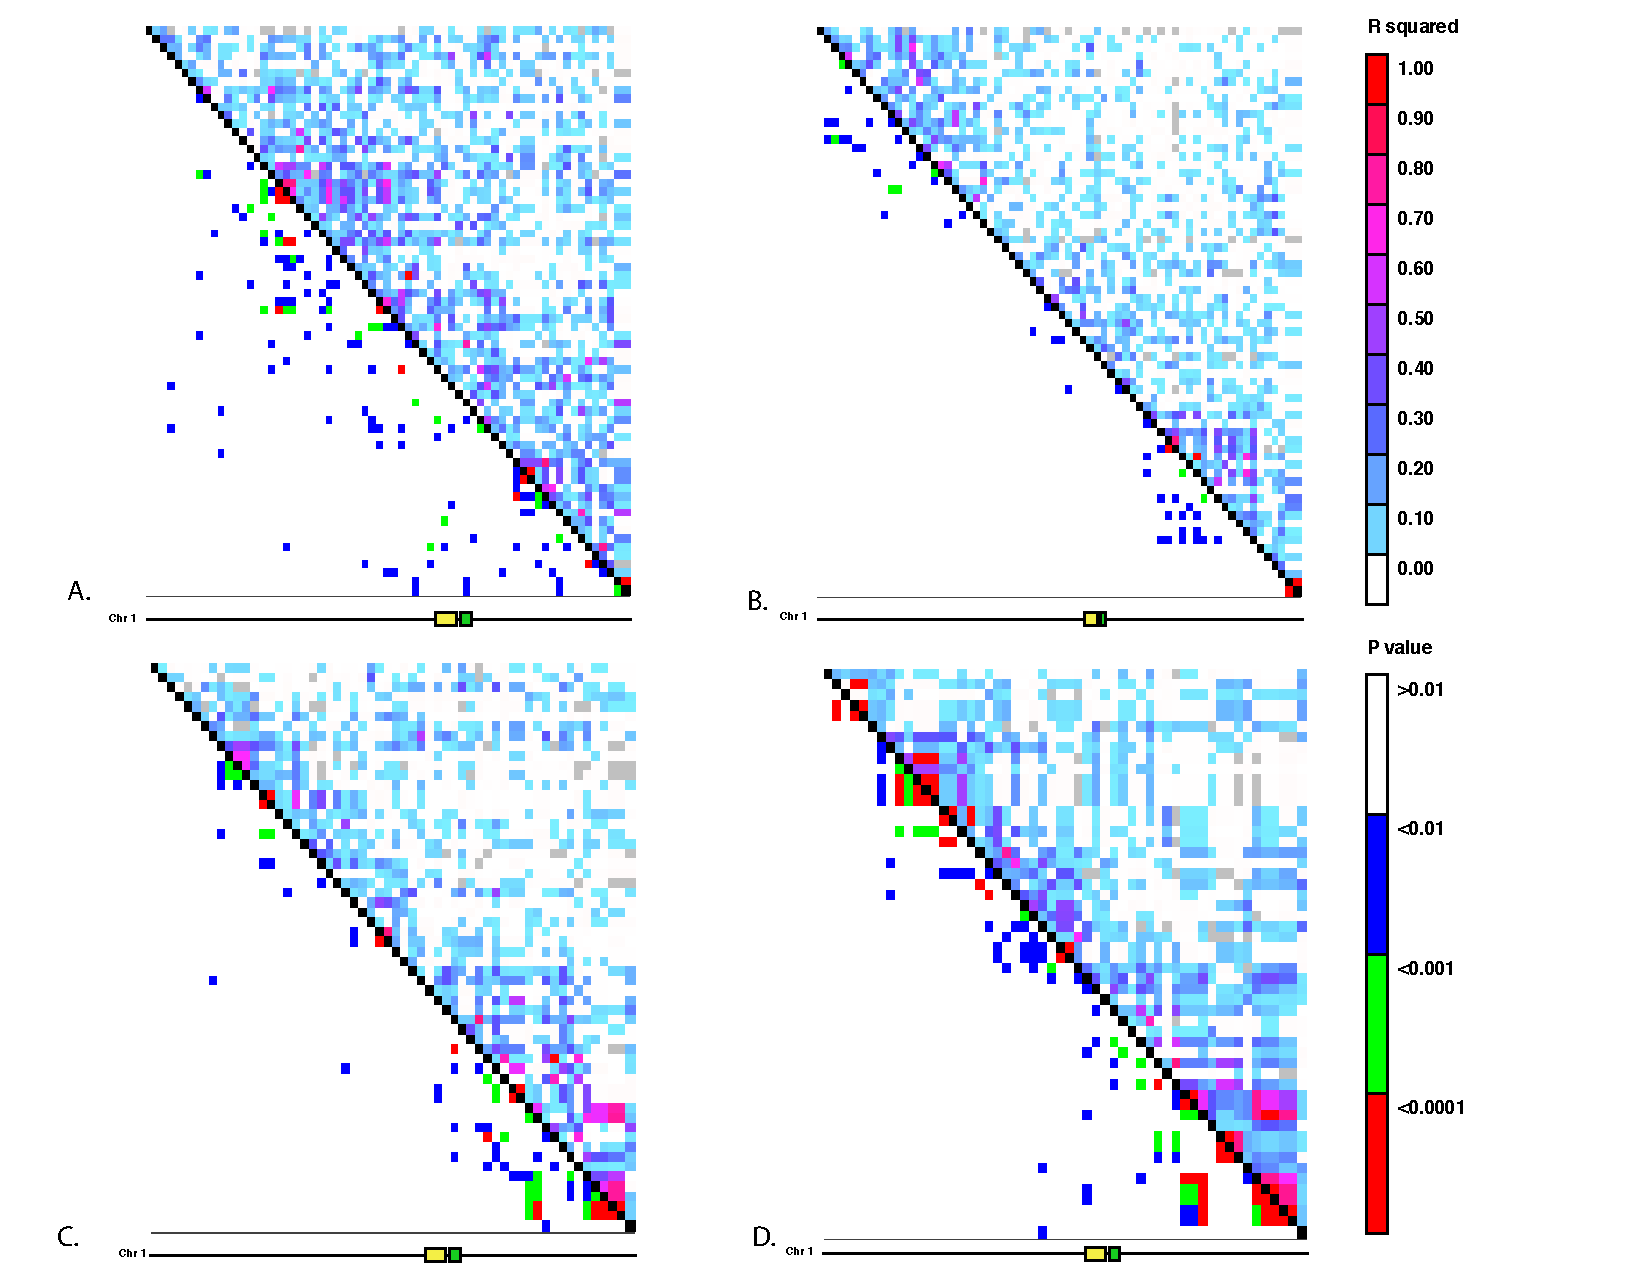
\includegraphics[width=140mm]{Fig2LDPlots.pdf}
    \caption{Linkage disequilibrium for SNPs in Mb 261-268 on chromosome 1. The yellow rectangle indicates the location of the \emph{Hopscotch} insertion and the green represents the \emph{tb1} ORF. A) Ejutla A; B) Ejutla B; C) La Mesa; D). San Lorenzo}  \jri{this needs description of what upper and lower triangle are}
\label{Fig2LD}
  \end{center}
\end{figure*}
%-------------------------------------------------------------------

The lack of clustering of \emph{Hopscotch} genotypes in our NJ tree as well as the lack of LD around \emph{tb1} does not support the hypothesis that the \emph{Hopscotch} insertion in these populations of \emph{parviglumis} is the result of recent introgression. However, to further explore this hypothesis we performed a STRUCTURE analysis using Illumina MaizeSNP50 data from four of our \emph{parviglumis} populations (EjuA, EjuB, MSA, and SLO) and the maize 282 diversity panel \citep{Cook2012, Pyhajarvi2013}. The linkage model implemented in STRUCTURE can be used to identify ancestry of blocks of linked variants, which would arise as a result of recent admixture between populations. If the \emph{Hopscotch} insertion is present in populations of \emph{parviglumis} as a result of recent admixture with domesticated maize, we would expect the insertion and linked variants in surrounding sites to be assigned to the "maize" cluster in our STRUCTURE runs, not the "teosinte" cluster. In all runs, assignment to maize in the \emph{tb1} region across all four \emph{parviglumis} populations is low (average 0.017) and much below the chromosome-wide average (0.20; Table \ref{Table4Q}; Fig. \ref{Fig3Structure}). 

 % Table 4 Assignment to maize and teosinte in tb1 region and chr 1 
\begin{table}[htbp]
\rowcolors{2}{gray!25}{white}
  \centering
  \caption{Assignments to maize and teosinte in the \emph{tb1} and chromosome 1 regions from STRUCTURE}
    \begin{tabular}{ccccc} \
          & \multicolumn{2}{c}{\textbf{\emph{tb1} region}} & \multicolumn{2}{c}{\textbf{Chr 1}} \\\toprule
    \bf{Population} & \bf{Maize} & \bf{Teosinte} & \bf{Maize} & \bf{Teosinte} \\\midrule
    Ejutla A & 0.022 & 0.978 & 0.203 & 0.797 \\
    Ejutla B & 0.019 & 0.981 & 0.187 & 0.813 \\
    La Mesa & 0.012 & 0.988 & 0.193 & 0.807 \\
    San Lorenzo & 0.016 & 0.984 & 0.205 & 0.795 \\\bottomrule
    \end{tabular}
  \label{Table4Q}
\end{table}

% Figure 3 STRUCTURE Plot 4 Pops
%-------------------------------------------------------------------
\begin{figure*}[!t]
  \begin{center}
   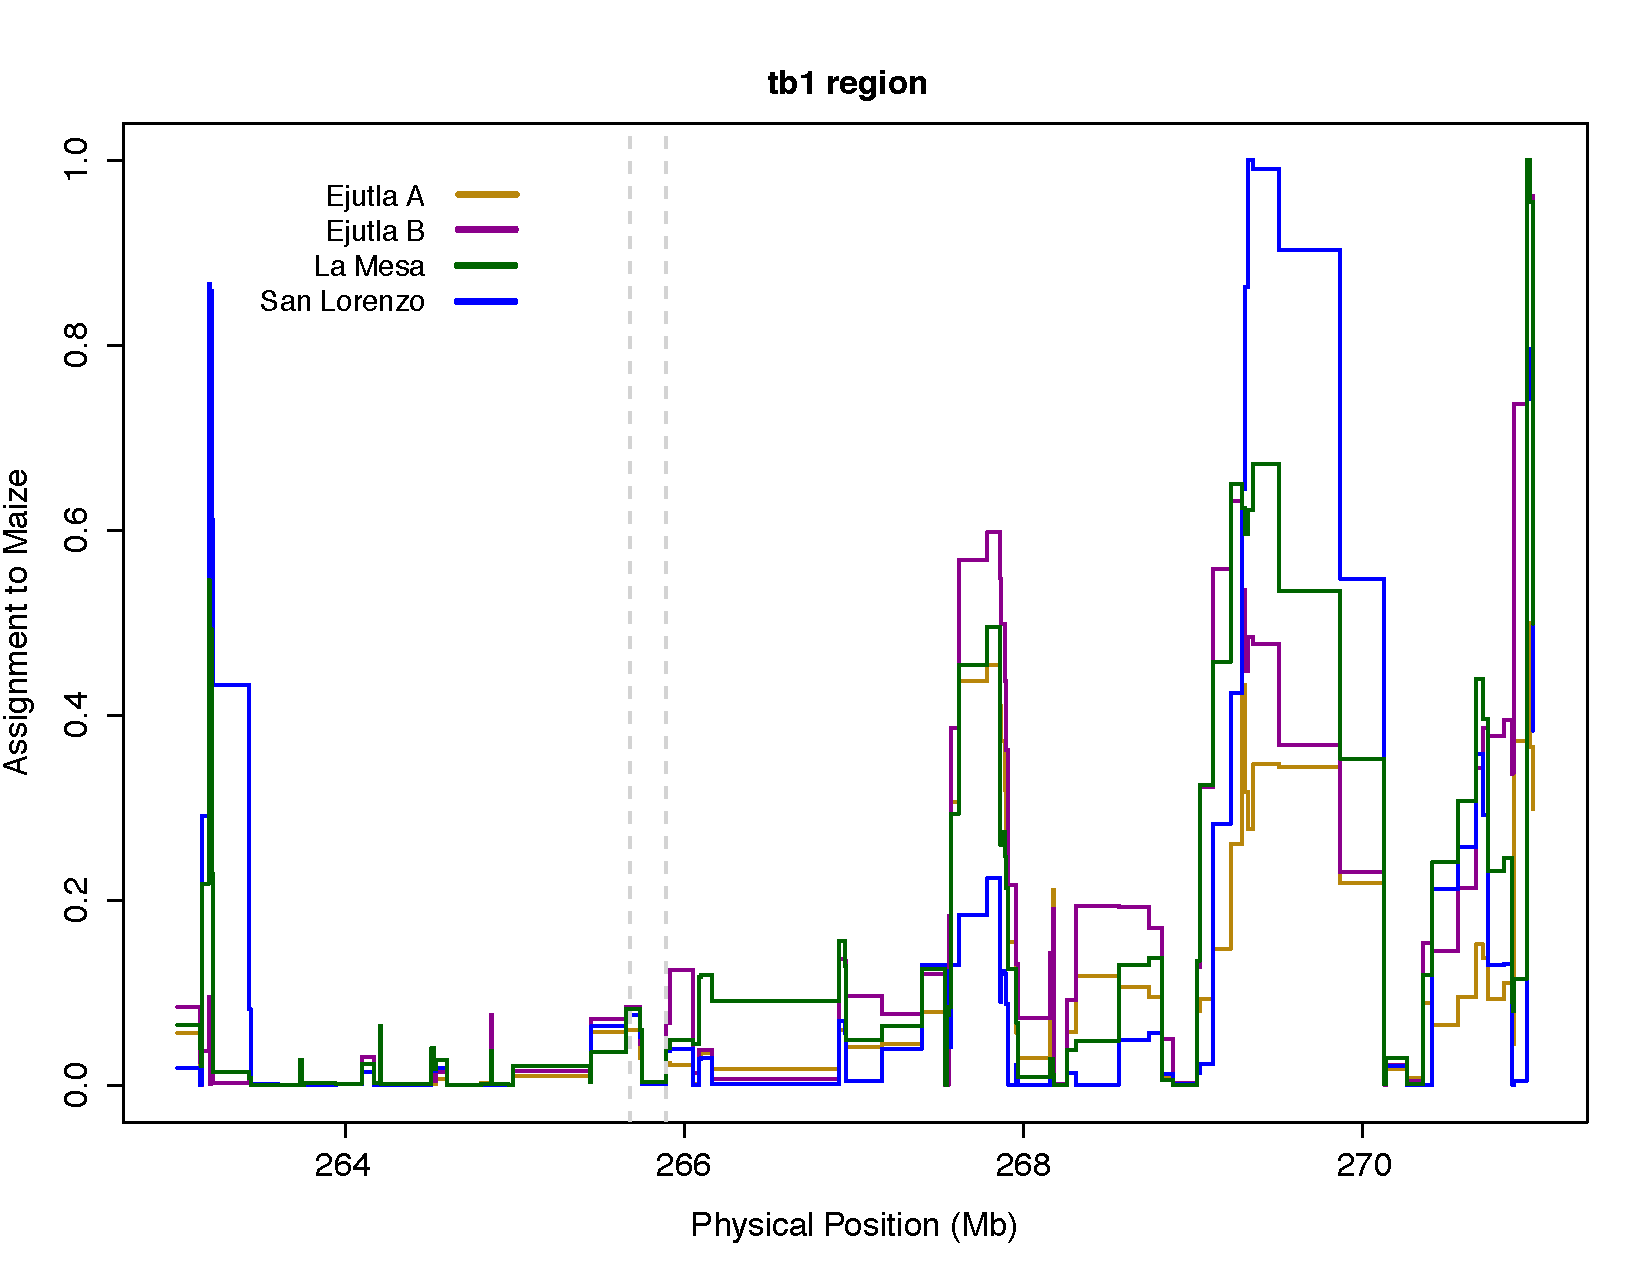
\includegraphics[width=90mm]{Fig3Structure.pdf}
    \caption{STRUCTURE assignment to maize across a section of chromosome 1. The dotted lines mark the beginning of the sequenced region 50kb upstream (Sequenced region 2) and the end of the \emph{tb1} ORF. } 
\label{Fig3Structure}
  \end{center}
\end{figure*}
%-------------------------------------------------------------------

\subsection*{Phenotyping}

To assess the contribution of \emph{tb1} to phenotypic variation in tillering in a natural population, we grew plants from seed sampled from the San Lorenzo population of \emph{parviglumis}, which had a high mean frequency (0.44) of the \emph{Hopscotch} insertion based on our initial genotyping. We measured tillering index (TI), the ratio of the sum of tiller lengths to plant height, for 216 plants (Phenotyping 1) from within the San Lorenzo population, and genotyped plants for the \emph{Hopscotch} insertion. We found the \emph{Hopscotch} segregating at a frequency of 0.65 with no significant deviations from expected frequencies under Hardy-Weinberg equilibrium. After performing a repeated measures ANOVA between our transformed tillering index data and \emph{Hopscotch} genotype we find a weak positive correlation between presence of the \emph{Hopscotch} and tillering index on day 40 (p=0.0848), a result indicating the \emph{Hopscotch} may actually increase tillering in \emph{parviglumis} in contrast to its phenotypic effect in maize. We find no correlation between tillering index and genotype on any other day (\ref{Fig4Boxplots}). Additionally we find no significant correlation between tiller number and \emph{Hopscotch} genotype, or culm diameter and \emph{Hopscotch} genotype in Phenotyping 1.

% Figure 4 Phenotyping BoxPlots
%-------------------------------------------------------------------
\begin{figure*}[!t]
  \begin{center}
   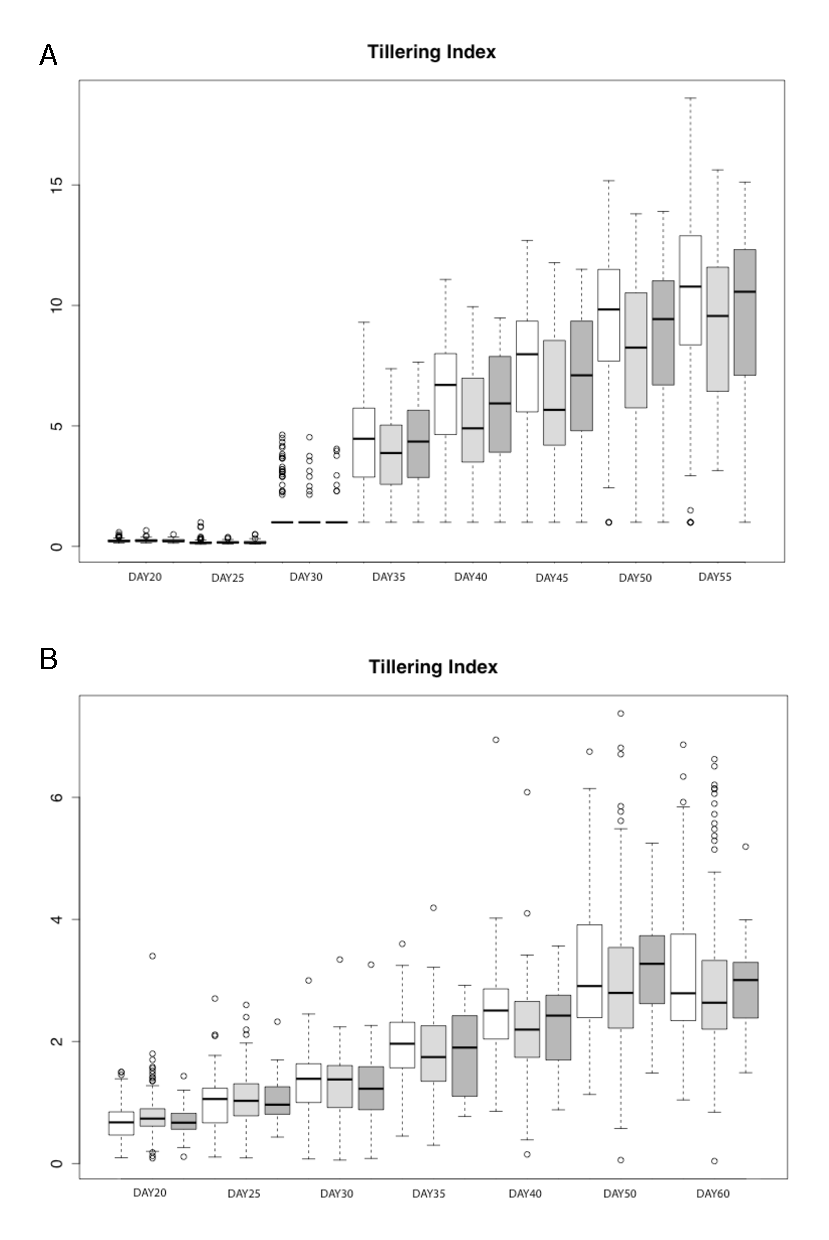
\includegraphics[width=95mm]{Fig4Boxplots.pdf}
    \caption{Box-plots showing tillering index in greenhouse grow-outs for Phenotyping 1 (A) and Phenotyping 2 (B). White indicates individuals homozygous for the \emph{Hopscotch}, light grey represents heterozygotes, and dark grey represents homozygotes for the teosinte (No \emph{Hopscotch}) allele. Within boxes, dark black lines represent the median, and the edges of the boxes are the first and third quartiles. \jri{please explain whiskers and dots on figure too.}} 
\label{Fig4Boxplots}
  \end{center}
\end{figure*}
%-------------------------------------------------------------------

We performed a second grow-out  of \emph{parviglumis} from San Lorenzo (Phenotyping 2) to assess whether lighting conditions or sample size may have affected our ability to detect an effect of \emph{tb1}.  For the second grow-out we measured tillering index every five days through day 50 for 302 plants. We found the \emph{Hopscotch} allele segregating at a frequency of 0.69, \jri{is it in HWE in this pop?} with a 0.6 frequency of \emph{Hopscotch} homozygotes, and a 0.2 frequency of both heterozygotes and homozygotes for the teosinte allele. We found similar patterns, with a weak positive correlation between tillering index and \emph{Hopscotch} genotype at day 40 (p$<$0.0611), with no significant correlation on any day. Similarly, relationships between \emph{Hopscotch} genotype and tiller number and \emph{Hopscotch} genotype and culm diameter were not significant. 

\begin{centering}
\section*{DISCUSSION}
\end{centering}

Adaptation occurs due to selection on standing variation or \emph{de novo} mutations. Adaptation from standing variation has been well-described in a number of systems; for example, selection for lactose tolerance in humans \citep{Plantinga2012, Tishkoff2007}, variation at the \emph{Eda} locus in three-spined stickleback \citep{Kitano2008, Colosimo2005}, and pupal diapause in the Apple Maggot fly \citep{Feder2003}. Although the adaptive role of standing variation has been described in many systems, its importance in domestication is not as well studied. 

In maize, alleles at domestication loci (\emph{RAMOSA1}, \citealt{SigmonVollbrecht2010}; \emph{barren stalk1}, \citealt{Gallavotti2004}; and \emph{grassy tillers1}, \citealt{Whipple2011}) are thought to have been selected from standing variation, suggesting that diversity already present in teosinte may have played an important role in maize domestication. The \emph{teosinte branched1} gene is one of the best characterized domestication loci, and, while previous studies have suggested that differences in plant architecture between maize and teosinte are a result of selection on standing variation at this locus, little is known about natural variation at this locus and its ecological role in teosinte \citep{Clark2006, Studer2011}. \citet{Studer2011} genotyped 90 accessions of teosinte (inbred and outbred), providing the first evidence that the \emph{Hopscotch} insertion is segregating in teosinte \citep{Studer2011}. 

Given that the \emph{Hopscotch} insertion has been estimated to predate the domestication of maize, it is not surprising that it can be found segregating in populations of teosinte. However, by widely sampling across teosinte populations our study provides greater insight into the distribution and prevalence of the \emph{Hopscotch} in teosinte. While our findings are consistent with \citet{Studer2011} in that we identify the \emph{Hopscotch} allele segregating in teosinte, we find it at higher frequency than previously suggested \citep{Studer2011}. Many of our populations with high frequency of the \emph{Hopscotch} allele fall in the Jalisco cluster identified by \citet{Fukunaga2005}, suggesting a different history of the \emph{tb1} locus in this region than in the Balsas River Basin where maize was domesticated \citep{Matsuoka2002}. Potential explanations for the high frequency of the \emph{Hopscotch} element in \emph{parviglumis} from the Jalisco cluster include gene flow from maize, genetic drift, and natural selection. 

While gene flow from crops into their wild relatives is well-known, \citep{Ellstrand1999, Zhang2009, Thurber2010, Baack2008, Hubner2012, Wilkes1977, VanHeerwaarden2011, Barrett1983}, our results are more consistent with \citet{Hufford2013} who found resistance to introgression from maize into teosinte. Furthermore, \citet{Hufford2013} showed that domestication loci, such as \emph{tb1}, are particularly resistant to introgression in both directions of gene flow (i.e., maize to teosinte and teosinte to maize). We find no evidence of recent introgression in our analyses. Clustering patterns in our NJ trees do not reflect a pattern expected if maize alleles at the \emph{tb1} locus had introgressed into populations of teosinte.  Moreover, there is no signature of elevated LD in the \emph{tb1} region relative to the rest of chromosome 1, and Bayesian assignment to a maize cluster in this region is lower than the chromosome-wide average (Fig. \ref{Fig3Structure}, Table \ref{Table4Q}). Together, these data point to an explanation other than recent introgression for the high observed frequency of \emph{Hopscotch} in a subset of our \emph{parviglumis} populations.

Although recent introgression seems unlikely, we cannot rule out ancient introgression as an explanation for the presence of the \emph{Hopscotch} in these populations. If the \emph{Hopscotch} allele was introgressed in the distant past, recombination may have broken up LD, a process that would be consistent with our data.  We find this scenario less plausible, however, as there is no reason why gene flow should have been high in the past but absent in present-day sympatric populations.  In fact, early generation maize-teosinte hybrids are common in these populations today (MB Hufford, pers. observation), and genetic data support ongoing gene flow between domesticated maize and both \emph{mexicana} and \emph{parviglumis} in a number of sympatric populations \citep{Hufford2013, Ellstrand2007, VanHeerwaarden2011}. 

Remaining explanations for differential frequencies of the \emph{Hopscotch} among teosinte populations include both genetic drift and natural selection.  Drift may have played a role in the San Lorenzo \emph{parviglumis} population. Previous studies using both SSRs and genome-wide SNP data have found evidence for a population bottleneck in the San Lorenzo population \citep{Hufford2010, Pyhajarvi2013}, and the lower levels of sequence diversity in this population in the 5' UTR (Region 1) coupled with more positive values of Tajima's D are consistent with these earlier findings suggesting a bottleneck. \jri{deviations from HWE may be consistent too if we see excess of homozygotes. do we?} Such population bottlenecks can exaggerate the effects of genetic drift through which the \emph{Hopscotch} allele may have risen to high frequency entirely by chance. This bottleneck, however, does not explain the high frequency of the \emph{Hopscotch} in multiple populations in the Jalisco cluster.  Moreover, available information on diversity and population structure among Jaliscan populations \citep{Hufford2010, Pyhajarvi2013} is not suggestive of recent colonization or other demographic events that would predict a high frequency of the allele across populations.  Finally, values of the Tajima's D statistic in the 5' UTR of \emph{tb1} are suggestive of natural selection acting upon the gene in natural population of \emph{parviglumis}.  Whereas the genome-wide average of Tajima's D in genic regions of \emph{parviglumis} is 0.45 \citep{Hufford2012b}, the statistic is quite negative in the 5' UTR of \emph{tb1} (Table \ref{Table2Diversity}). This result is consistent with repeated selective sweeps near \emph{tb1} and a putative ecological role for the gene in \emph{parviglumis}.

\jri{do we know the Hop genotype for sequenced lines? can we separate the sequences into hop/no hop and look for differences? it wasn't until we did this that gt1 stuff really popped out.} \lev{we should know for some of them, i will check} \mbh{I've added a few sentences on selection.  Do we still want to compare sequences with and without \emph{Hopscotch}?  I agree its a good idea and could end up being really interesting.  Perhaps something we could look at after submission and incorporate during revisions?}

Significant effects of the \emph{Hopscotch} insertion on lateral branch length, number of cupules, and tillering index in domesticated maize have been well documented \citep{Studer2011}.  \citet{Weber2007} have described significant phenotypic associations between markers in and around \emph{tb1} and lateral branch length and female ear length in a sample from 74 natural populations of \emph{parviglumis} \citep{Weber2007}; however, these data did not include markers from the \emph{Hopscotch} region 66kb upstream of \emph{tb1}. Our study is the first to explicitly examine the phenotypic effects of the \emph{Hopscotch} insertion across a wide collection of individuals sampled from natural populations of teosinte. We have found no significant effect of the \emph{Hopscotch} insertion on tillering index or tiller number, a result that is discordant with its clear phenotypic effects in maize. One interpretation of this result would be that the \emph{Hopscotch} controls tillering in maize \citep{Studer2011}, but tillering in teosinte is affected by variation at other loci. Consistent with this interpretation, \emph{tb1} is thought to be part of a complex pathway controlling branching, tillering and other phenotypic traits \citep{KebromBrutnell2007, Clark2006}. A recent study by \citet{StuderDoebley2012} examined variation across traits in a three-taxa allelic series at the \emph{tb1} locus. \citet{StuderDoebley2012} introgressed nine unique teosinte \emph{tb1} segments (one from \emph{Zea diploperennis}, and four each from \emph{mexicana} and \emph{parviglumis}) into an inbred maize background and investigated phenotypic effects. Phenotypes were shown to cluster by taxon, indicating \emph{tb1} may underlie morphological diversification of \emph{Zea}. Additional analysis in \citet{StuderDoebley2012} suggested tillering index was controlled both by \emph{tb1} and loci elsewhere in the genome.  Clues to the identity of these loci may be found in QTL studies that have identified loci controlling branching architecture (\emph{e.g.,} \citealt{DoebleyStec1991, DoebleyStec1993}). Many of these loci (\emph{grassy tillers}, \emph{gt1}; \emph{tassel-replaces-upper-ears1}, \emph{tru1}; \emph{terminal ear1}, \emph{ter1}) have been shown to interact with \emph{tb1} \citep{Whipple2011, Li2012},  and both \emph{tru1} and \emph{ter1} affect the same phenotypic traits as \emph{tb1} \citep{DoebleyStecGustus1995}. \emph{tassel-replaces-upper-ears1} (\emph{tru1}), for example, has been shown to act either epistatically or downstream of \emph{tb1}, affecting both branching architecture (decreased apical dominance) and tassel phenotypes (shortened tassel and shank length and reduced tassel number; \citealt{Li2012}). Variation in these additional loci may have affected tillering in our collections and contributed to the lack of correlation we see between \emph{Hopscotch} genotype and tillering. 

In conclusion, our findings demonstrate that the \emph{Hopscotch} allele is more widespread in populations of \emph{parviglumis} and \emph{mexicana} than previously thought. Analysis of linkage using SNPs from across chromosome 1 does not suggest that the \emph{Hopscotch} allele is present in these populations due to recent introgression; however, it seems unlikely that the insertion would have drifted to high frequency in multiple populations. We do, however, find preliminary evidence of selection on the \emph{tb1} locus in \emph{parviglumis}; this coupled with our observation of high frequency of the \emph{Hopscotch} insertion in a number of populations suggests that the locus plays an ecological role in teosinte. In contrast to domesticated maize, the \emph{Hopscotch} insertion in \emph{parviglumis} does not appear to reduce tillering. Other loci involved in branching architecture may regulate tillering in teosinte. Future studies should examine expression levels of \emph{tb1} in teosinte with and without the \emph{Hopscotch} insertion and further characterize the effects of additional loci involved in branching architecture (e.g. \emph{gt1}, \emph{tru1}, and \emph{ter1}).  These data, in conjunction with more exhaustive phenotyping, should help reveal the ecological significance of the domesticated \emph{tb1} allele in natural populations of teosinte. \jri{why not Phyb and phya? } \lev{Are they necessary to include? I'd had them in before in a paragraph but had been voted out} \jri{I'd ditch gt1 tru1 ter1 and maybe just cite some people including phyb etc.}

\jri{please check format of supp figs and tables; some are running off the page.  you can use "longtable" to fix that (ask Paul for example). check fig/table references, bibliography, etc. what does "rotation" mean in supp. table 3? it isn't mentioned in methods. please check that all the tables and figs (including supplement) are referenced in the text.}

%\jri{seems like we should end with at least a hypothesis. as is we are saying we ruled out drift, introgression, and selection. what else is there? perhaps we should think about selection or introgression scenarios that could explain our data.} 

%\mbh{I'd lean toward saying that 1) \emph{Hopscotch} does not appear to uniformly reduce tillering in teosinte as it seems to in maize; 2) other loci are likely involved in regulating tillering; 3) given its high frequency in several teosinte populations, \emph{Hopscotch} may play additional ecological roles not obvious here based on what we chose to phenotype and, in the future,  additional experiments are needed to look at 1) expression level differences at various loci shown to affect tillering in teosinte; and 2) to more completely phenotype teosinte plants with and without the \emph{Hopscotch}.}

%\lev{I went with Matt's suggestions. I am happy to include such scenarios, but everything I have thought of seems rather unlikely; i.e. only introgression or selection in Jalisco. Jeff I can mention that maybe parv is more of a weed there than other locations, but i thought that maize pollen spread rather substantial distances. If so wouldn't a number of our parv and mex sites would be within pollen dispersal distance?}

\clearpage
\bibliography{refs,bob}

%-------------------------------------------------
Supplementary Materials
%-------------------------------------------------
\clearpage
\setcounter{figure}{0}
\setcounter{table}{0}
\renewcommand{\figurename}{Sup.\Fig.}
\renewcommand{\tablename}{Sup.\Table}

% Figure S1. Cartoon representation of tb1 locus
%-------------------------------------------------------------------
\begin{figure*}[!t]
  \begin{center}
   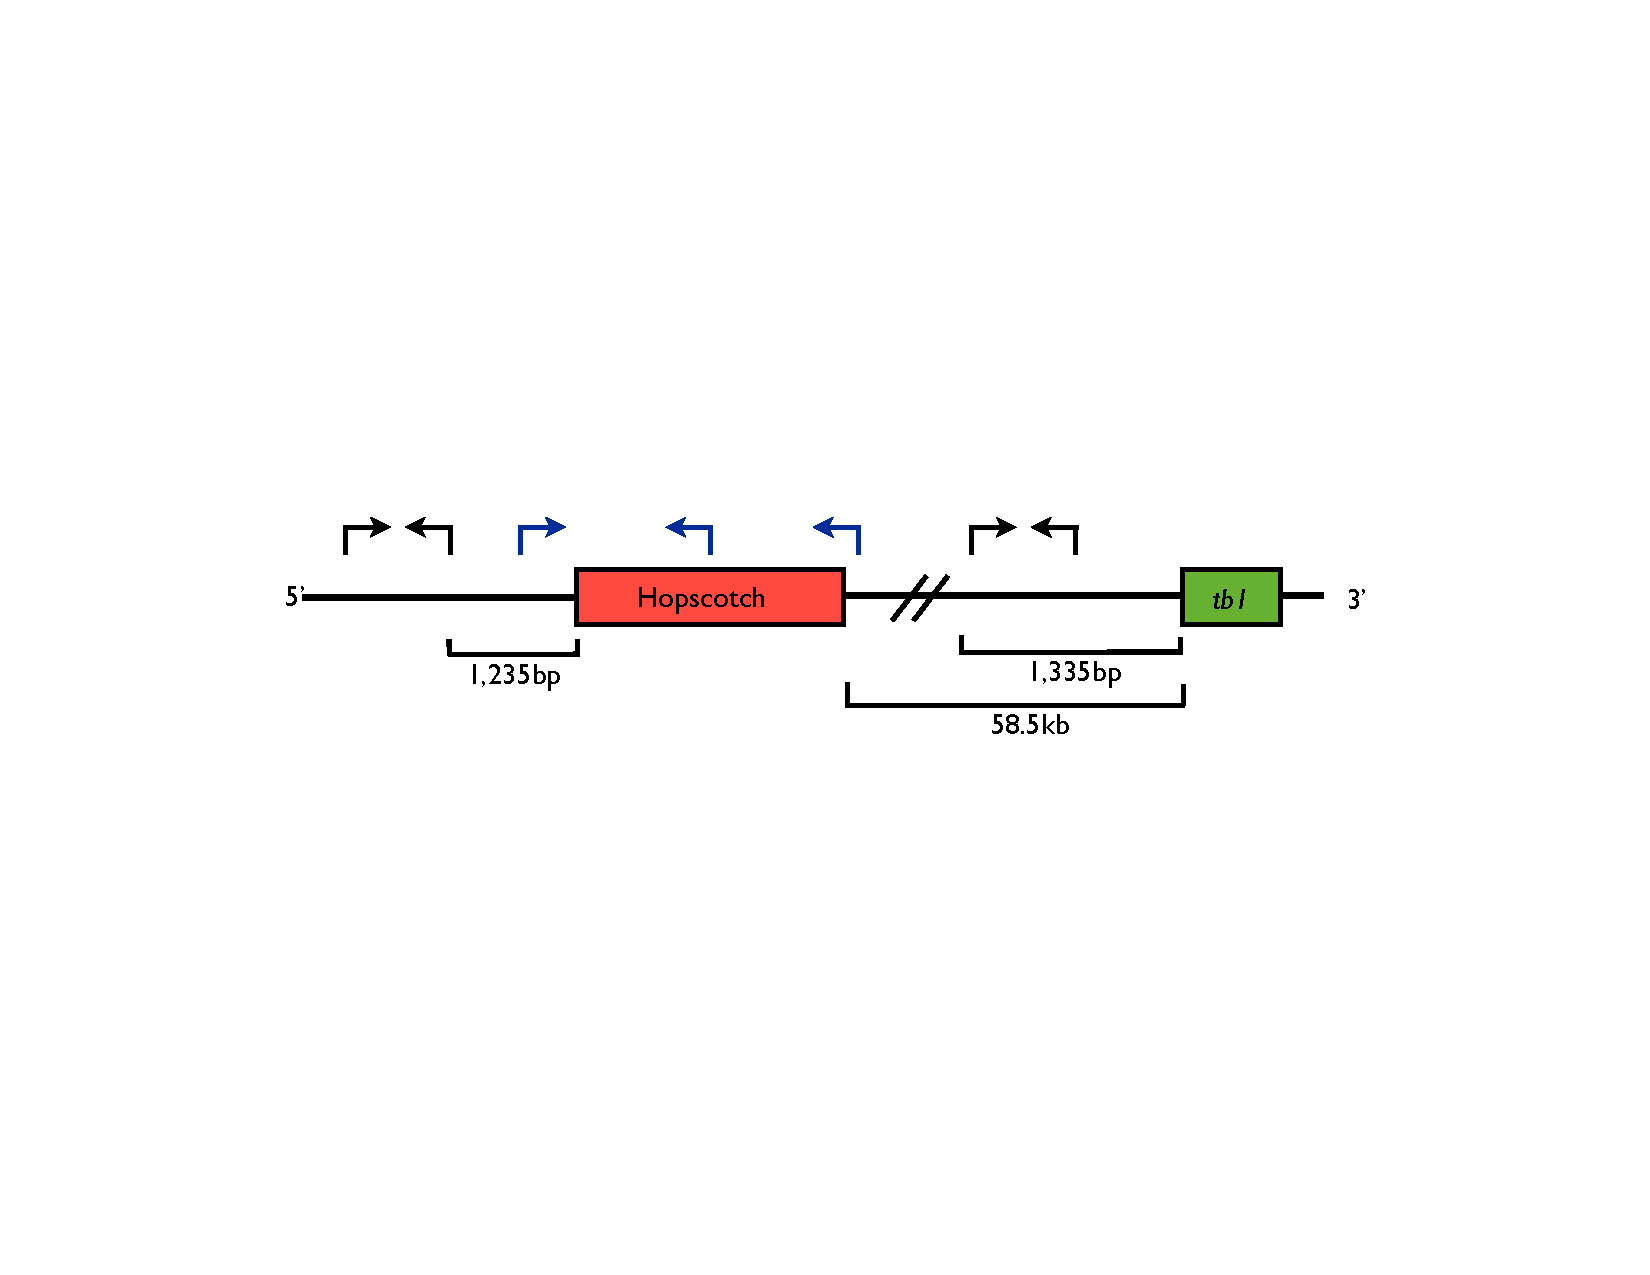
\includegraphics[width=150mm]{FigS1LocusCartoon.pdf}
   % \caption{Representation of the upstream regulatory region of \emph{tb1}, showing the \emph{tb1} coding region (green) and the \emph{Hopscotch} insertion (red). Arrows show the location of primer sets; in black, primers used for amplification and sequencing (Sequenced region 1; within the 5' UTR, and sequenced region 2; 66,169 bp upstream from the tb1 ORF); in blue, primers used to genotype the \emph{Hopscotch} insertion.}
\label{FigS1Locus}
  \end{center}
\end{figure*}
%-------------------------------------------------------------------

% Figure S2. Gel image
%-------------------------------------------------------------------
\begin{figure*}[!t]
  \begin{center}
   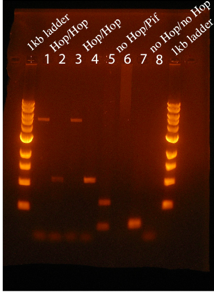
\includegraphics[width=150mm]{FigS2Gel.png}
   % \caption{Agarose gel image of amplification products using our primer sets. Genotypes are indicated at the top of the gel.} 
\label{FigS2Gel}
  \end{center}
\end{figure*}
%-------------------------------------------------------------------

% Figure S3. NJ Trees
%-------------------------------------------------------------------
\begin{figure*}[!t]
  \begin{center}
   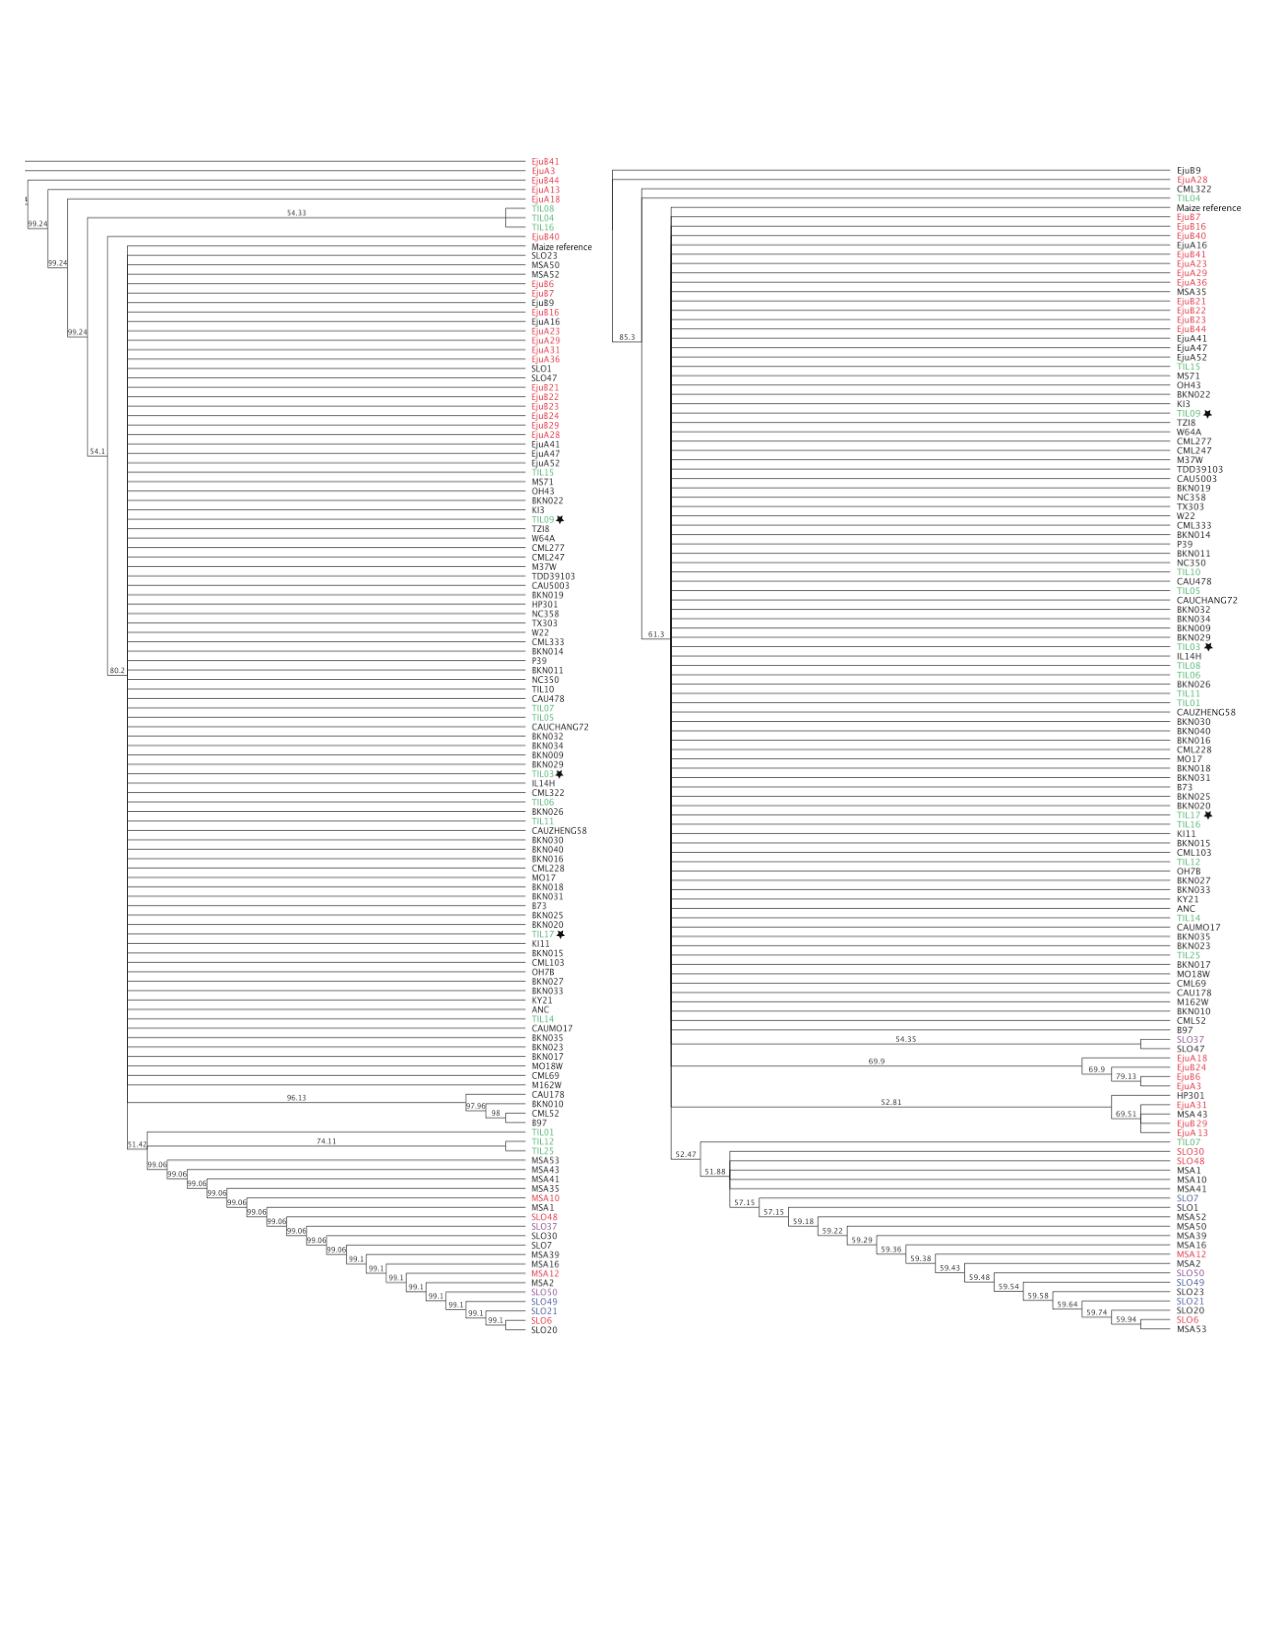
\includegraphics[width=150mm]{FigS3NJtrees.pdf}
    %\caption{Neighbor-Joining tree of the sequenced region in the 5? UTR (right; sequenced region 1) and the 66,169 bp upstream region (left; sequenced region 2) of \emph{tb1}. Individuals with genotype data are colored: Homozygous for the teosinte (no \emph{Hopscotch}) allele (red), homozygous for the maize (\emph{Hopscotch}) allele (blue), heterozygotes (purple). TILs (teosinte inbred lines) are colored in green, with stars indicating the 3 TILs known to have the \emph{Hopscotch} insertion. Black indicates individuals not genotyped for the \emph{Hopscotch} insertion.} 
\label{FigS3NJ}
  \end{center}
\end{figure*}
%-------------------------------------------------------------------

% Table S1. Parv and mex samples
\begin{table}[htbp]
  \centering
  %\caption{Accessions of \emph{Zea mays} ssp. \emph{mexicana} (RIMME) and \emph{Zea mays} ssp. \emph{parviglumis} (RIMPA) sampled. RIHY is a \emph{Z. mays} ssp. \emph{parviglumis} and \emph{Zea mays} ssp. \emph{mays} hybrid. }
    \begin{tabular}{rrrrrr}
%    \toprule
    Accession & USDA Accession ID & Locality & Number alleles sampled & \emph{Hopscotch} Frequency & No \emph{Hopscotch} Frequency \\
 %   \midrule
    RIHY0009 & N/A   & N/A   & 2     & 0.5   & 0.5 \\
    RIMME0006 & 566673 & Durango, Mexico & 2     & 0     & 1 \\
    RIMME0007 & 566680 & Guanajuato, Mexico & 2     & 0     & 1 \\
    RIMME0008 & 566681 & Michoacan, Mexico & 2     & 0     & 1 \\
    RIMME0009 & 566682 & Distrito Federal, Mexico & 2     & 0     & 1 \\
    RIMME0011 & 566685 & Mexico, Mexico & 2     & 0     & 1 \\
    RIMME0014 & 714151 & Breeders line; Puga: 11066 & 6     & 0     & 1 \\
    RIMME0017 & 699874 & Ayotlan, Mexico & 8     & 0     & 1 \\
    RIMME0021 & N/A   & El Porvenir, Mexico & 69    & 0.173913043 & 0.826086957 \\
    RIMME0026 & N/A   & Opopeo, Mexico & 42    & 0.071428571 & 0.928571429 \\
    RIMME0028 & N/A   & Puruandiro, Mexico & 28    & 0.035714286 & 0.964285714 \\
    RIMME0029 & N/A   & Ixtlan, Mexico & 35    & 0     & 1 \\
    RIMME0030 & N/A   & San Pedro, Mexico & 27    & 0     & 1 \\
    RIMME0031 & N/A   & Tenango del Aire, Mexico & 25    & 0.08  & 0.92 \\
    RIMME0032 & N/A   & Nabogame, Mexico & 24    & 0     & 1 \\
    RIMME0033 & N/A   & Puerta Encantada, Mexico & 25    & 0     & 1 \\
    RIMME0034 & N/A   & Santa Clara, Mexico & 23    & 0     & 1 \\
    RIMME0035 & N/A   & Xochimilco, Mexico & 25    & 0     & 1 \\
    RIMPA0001 & 87168 & El Salado, Mexico & 4     & 0     & 1 \\
    RIMPA0003 & 87171 & Mazatlan, Mexico & 8     & 0.125 & 0.875 \\
    RIMPA0017 & 87200 & N/A   & 4     & 0     & 1 \\
    RIMPA0019 & 87213 & El Salado, Mexico & 2     & 0.5   & 0.5 \\
    RIMPA0029 & 87244 & N/A   & 2     & 0.5   & 0.5 \\
    RIMPA0031 & 87249 & N/A   & 2     & 0.5   & 0.5 \\
    RIMPA0035 & 87288 & Jalisco, Mexico & 4     & 0     & 1 \\
    RIMPA0040 & 288185 & Mexico, Mexico & 4     & 0     & 1 \\
    RIMPA0042 & 288187 & Guerrero, Mexico & 4     & 0.25  & 0.75 \\
    RIMPA0043 & 288188 & Guerrero, Mexico & 4     & 0     & 1 \\
    RIMPA0045 & 288193 & Guerrero, Mexico & 4     & 0     & 1 \\
    RIMPA0055 & 714152 & Breeders line & 2     & 0     & 1 \\
    RIMPA0056 & 714153 & Breeders line & 2     & 0.5   & 0.5 \\
    RIMPA0057 & 714154 & Breeders line & 2     & 0.5   & 0.5 \\
    RIMPA0058 & N/A   & N/A   & 4     & 0.5   & 0.5 \\
    RIMPA0059 & N/A   & N/A   & 4     & 1     & 0 \\
    RIMPA0060 & 714157 & Breeders line: CIMMYT 11355 & 2     & 0     & 1 \\
    RIMPA0061 & 714158 & Breeders line: USDA PI566686 & 4     & 0.5   & 0.5 \\
    RIMPA0062 & 714159 & Breeders line & 4     & 0.5   & 0.5 \\
    RIMPA0063 & 714160 & Breeders line & 4     & 0     & 1 \\
    RIMPA0064 & 714161 & Breeders line & 3     & 0     & 1 \\
    RIMPA0065 & 714162 & Breeders line & 4     & 0.25  & 0.75 \\
    RIMPA0068 & 699861 & Jalisco, Mexico & 16    & 0     & 1 \\
    RIMPA0069 & 699862 & Ixtlan, Mexico & 14    & 0.142857143 & 0.857142857 \\
    RIMPA0070 & 699863 & Benito Jaurez, Mexico & 16    & 0     & 1 \\
    RIMPA0071 & 699864 & Tuzantla, Mexico & 28    & 0     & 1 \\
    RIMPA0072 & 699865 & Tiquicheo, Mexico & 16    & 0     & 1 \\
    RIMPA0073 & 699866 & Tiquicheo, Mexico & 16    & 0.125 & 0.875 \\
    RIMPA0074 & 699867 & Huetamo, Mexico & 12    & 0     & 1 \\
    RIMPA0075 & 699868 & Huetamo, Mexico & 2     & 0     & 1 \\
    RIMPA0076 & 699869 & Huetamo, Mexico & 4     & 0     & 1 \\
    RIMPA0077 & 699870 & Caracuaro, Mexico & 2     & 0     & 1 \\
    RIMPA0078 & 699871 & Caracuaro, Mexico & 2     & 0.5   & 0.5 \\
    RIMPA0079 & 699872 & Villa Madero, Mexico & 14    & 0     & 1 \\
    RIMPA0080 & 699873 & Guachinango, Mexico & 12    & 0     & 1 \\
    RIMPA0081 & 699875 & Ameca, Mexico & 16    & 0     & 1 \\
    RIMPA0083 & 699877 & Tepoztlan, Mexico & 14    & 0     & 1 \\
    RIMPA0084 & 699878 & Tepoztlan, Mexico & 16    & 0     & 1 \\
    RIMPA0085 & 699879 & Miahuatlan, Mexico & 16    & 0     & 1 \\
    RIMPA0086 & 699880 & Miahuatlan, Mexico & 16    & 0.0625 & 0.9375 \\
    RIMPA0087 & 699881 & Tecoanapa, Mexico & 24    & 0     & 1 \\
    RIMPA0089 & 699883 & Guerrero, Mexico & 12    & 0     & 1 \\
    RIMPA0090 & 699884 & Guerrero, Mexico & 10    & 0     & 1 \\
    RIMPA0091 & 699885 & Guerrero, Mexico & 16    & 0     & 1 \\
    RIMPA0092 & 699886 & Guerrero, Mexico & 10    & 0     & 1 \\
    RIMPA0093 & 699887 & Guerrero, Mexico & 26    & 0.076923077 & 0.923076923 \\
    RIMPA0094 & 699888 & Guerrero, Mexico & 2     & 0     & 1 \\
    RIMPA0095 & 699889 & Guerrero, Mexico & 4     & 0     & 1 \\
    RIMPA0096 & 699890 & Guerrero, Mexico & 26    & 0.038461538 & 0.961538462 \\
    RIMPA0097 & 699891 & Guerrero, Mexico & 6     & 0     & 1 \\
    RIMPA0098 & 699892 & Guerrero, Mexico & 4     & 0     & 1 \\
    RIMPA0099 & 699893 & Guerrero, Mexico & 4     & 0     & 1 \\
    RIMPA0100 & 699894 & Guerrero, Mexico & 6     & 0     & 1 \\
    RIMPA0101 & 699895 & Guerrero, Mexico & 2     & 0     & 1 \\
    RIMPA0103 & 699897 & Guerrero, Mexico & 2     & 0     & 1 \\
    RIMPA0104 & 699898 & Guerrero, Mexico & 22    & 0.090909091 & 0.909090909 \\
    RIMPA0105 & 699899 & Guerrero, Mexico & 6     & 0     & 1 \\
    RIMPA0106 & 699900 & Guerrero, Mexico & 6     & 0.333333333 & 0.666666667 \\
    RIMPA0107 & 699901 & Guerrero, Mexico & 4     & 0     & 1 \\
    RIMPA0108 & 699902 & Guerrero, Mexico & 6     & 0     & 1 \\
    RIMPA0109 & 699903 & Michoacan, Mexico & 4     & 0.25  & 0.75 \\
    RIMPA0110 & 699904 & Michoacan, Mexico & 2     & 0     & 1 \\
    RIMPA0111 & 699905 & Michoacan, Mexico & 4     & 0     & 1 \\
    RIMPA0112 & 699906 & Michoacan, Mexico & 4     & 0.25  & 0.75 \\
    RIMPA0114 & 699908 & Michoacan, Mexico & 6     & 0.166666667 & 0.833333333 \\
    RIMPA0116 & 699910 & Mexico, Mexico & 2     & 0     & 1 \\
    RIMPA0117 & 699911 & Mexico, Mexico & 4     & 0     & 1 \\
    RIMPA0118 & 699912 & Mexico, Mexico & 6     & 0.166666667 & 0.833333333 \\
    RIMPA0119 & 699913 & Mexico, Mexico & 2     & 0     & 1 \\
    RIMPA0120 & 699914 & Mexico, Mexico & 1     & 1     & 0 \\
    RIMPA0121 & 699915 & Mexico, Mexico & 2     & 0     & 1 \\
    RIMPA0128 & 699922 & Mexico, Mexico & 2     & 0.5   & 0.5 \\
    RIMPA0129 & 699923 & Michoacan, Mexico & 2     & 0.5   & 0.5 \\
    RIMPA0135 & 699929 & Nayarit, Mexico & 24    & 0     & 1 \\
    RIMPA0138 & 699932 & Jalisco, Mexico & 2     & 0.5   & 0.5 \\
    RIMPA0139 & 699933 & Jalisco, Mexico & 1     & 1     & 0 \\
    RIMPA0142 & 699936 & Colima, Mexico & 18    & 0.444444444 & 0.555555556 \\
    RIMPA0144 & 699938 & Jalisco, Mexico & 2     & 1     & 0 \\
    RIMPA0145 & 699939 & Michoacan, Mexico & 1     & 1     & 0 \\
    RIMPA0147 & 699941 & Jalisco, Mexico & 1     & 1     & 0 \\
    RIMPA0155 & N/A   & Jalisco, Mexico & 73    & 0.01369863 & 0.98630137 \\
    RIMPA0156 & N/A   & Jalisco, Mexico & 20    & 0     & 1 \\
    RIMPA0157 & N/A   & Jalisco, Mexico & 58    & 0.344827586 & 0.655172414 \\
    RIMPA0158 & N/A   & Jalisco, Mexico & 64    & 0.53125 & 0.46875 \\
    RIMPA0159 & N/A   & Jalisco, Mexico & 26    & 0     & 1 \\
    RIMPA0162 & 21785 & N/A   & 4     & 0     & 1 \\
 %   \bottomrule
    \end{tabular}
  \label{TableS1}
\end{table}

% Table S2. Mays sampling
\begin{table}[htbp]
  \centering
 % \caption{\emph{Zea mays} ssp. \emph{mays} (RIMMA) sampled for genotyping}
    \begin{tabular}{ccc}
 %   \toprule
    Accession & Number of alleles sampled & \emph{Hopscotch} Frequency \\
 %   \midrule
    RIMMA0066 & 2     & 1 \\
    RIMMA0075 & 2     & 1 \\
    RIMMA0077 & 2     & 1 \\
    RIMMA0079 & 2     & 1 \\
    RIMMA0081 & 2     & 1 \\
    RIMMA0084 & 2     & 1 \\
    RIMMA0086 & 2     & 1 \\
    RIMMA0088 & 2     & 1 \\
    RIMMA0089 & 2     & 1 \\
    RIMMA0090 & 2     & 1 \\
    RIMMA0092 & 4     & 1 \\
    RIMMA0094 & 4     & 1 \\
    RIMMA0097 & 2     & 1 \\
    RIMMA0099 & 2     & 1 \\
    RIMMA0100 & 2     & 1 \\
    RIMMA0101 & 2     & 1 \\
    RIMMA0104 & 2     & 1 \\
    RIMMA0108 & 2     & 1 \\
    RIMMA0111 & 6     & 1 \\
    RIMMA0115 & 2     & 1 \\
    RIMMA0117 & 2     & 1 \\
    RIMMA0130 & 2     & 1 \\
    RIMMA0133 & 2     & 1 \\
    RIMMA0134 & 2     & 1 \\
    RIMMA0135 & 2     & 1 \\
    RIMMA0142 & 2     & 0.5 \\
    RIMMA0143 & 4     & 1 \\
    RIMMA0146 & 4     & 1 \\
    RIMMA0149 & 2     & 1 \\
    RIMMA0152 & 2     & 1 \\
    RIMMA0153 & 2     & 1 \\
    RIMMA0154 & 2     & 1 \\
    RIMMA0155 & 2     & 1 \\
    RIMMA0156 & 2     & 1 \\
    RIMMA0157 & 2     & 1 \\
    RIMMA0158 & 2     & 1 \\
    RIMMA0159 & 2     & 1 \\
    RIMMA0160 & 2     & 1 \\
    RIMMA0162 & 2     & 1 \\
    RIMMA0166 & 2     & 1 \\
    RIMMA0167 & 2     & 1 \\
    RIMMA0168 & 2     & 1 \\
    RIMMA0169 & 2     & 1 \\
    RIMMA0172 & 2     & 1 \\
    RIMMA0174 & 4     & 1 \\
    RIMMA0177 & 2     & 1 \\
    RIMMA0178 & 2     & 1 \\
    RIMMA0179 & 2     & 1 \\
    RIMMA0181 & 2     & 1 \\
    RIMMA0183 & 2     & 1 \\
    RIMMA0184 & 2     & 1 \\
    RIMMA0186 & 2     & 1 \\
    RIMMA0187 & 1     & 1 \\
    RIMMA0188 & 2     & 1 \\
    RIMMA0195 & 2     & 1 \\
    RIMMA0196 & 2     & 1 \\
    RIMMA0197 & 2     & 1 \\
    RIMMA0198 & 2     & 1 \\
    RIMMA0199 & 2     & 1 \\
    RIMMA0200 & 2     & 1 \\
    RIMMA0202 & 2     & 1 \\
    RIMMA0203 & 2     & 1 \\
    RIMMA0206 & 2     & 1 \\
    RIMMA0208 & 2     & 1 \\
    RIMMA0209 & 2     & 1 \\
    RIMMA0210 & 2     & 1 \\
    RIMMA0212 & 2     & 1 \\
    RIMMA0213 & 2     & 1 \\
    RIMMA0214 & 2     & 1 \\
    RIMMA0217 & 2     & 1 \\
    RIMMA0218 & 2     & 1 \\
    RIMMA0220 & 2     & 1 \\
    RIMMA0221 & 2     & 1 \\
    RIMMA0222 & 2     & 1 \\
    RIMMA0223 & 2     & 1 \\
    RIMMA0226 & 2     & 1 \\
    RIMMA0227 & 2     & 1 \\
    RIMMA0228 & 2     & 1 \\
    RIMMA0229 & 2     & 1 \\
    RIMMA0230 & 2     & 1 \\
    RIMMA0232 & 2     & 1 \\
    RIMMA0233 & 2     & 1 \\
    RIMMA0235 & 2     & 0.5 \\
    RIMMA0242 & 2     & 1 \\
    RIMMA0243 & 2     & 1 \\
    RIMMA0247 & 4     & 1 \\
    RIMMA0248 & 2     & 1 \\
    RIMMA0249 & 2     & 1 \\
    RIMMA0252 & 2     & 1 \\
    RIMMA0253 & 2     & 1 \\
    RIMMA0254 & 2     & 1 \\
    RIMMA0256 & 2     & 1 \\
    RIMMA0257 & 2     & 1 \\
    RIMMA0258 & 2     & 1 \\
    RIMMA0259 & 2     & 1 \\
    RIMMA0260 & 2     & 1 \\
    RIMMA0262 & 2     & 1 \\
    RIMMA0263 & 2     & 1 \\
    RIMMA0264 & 2     & 1 \\
    RIMMA0265 & 2     & 1 \\
    RIMMA0268 & 2     & 1 \\
    RIMMA0269 & 2     & 1 \\
    RIMMA0270 & 2     & 1 \\
    RIMMA0272 & 2     & 1 \\
    RIMMA0275 & 2     & 1 \\
    RIMMA0276 & 2     & 1 \\
    RIMMA0277 & 2     & 1 \\
    RIMMA0279 & 2     & 1 \\
    RIMMA0280 & 2     & 1 \\
    RIMMA0283 & 2     & 1 \\
    RIMMA0285 & 2     & 1 \\
    RIMMA0288 & 2     & 1 \\
    RIMMA0290 & 2     & 1 \\
    RIMMA0291 & 2     & 1 \\
    RIMMA0292 & 2     & 1 \\
    RIMMA0293 & 2     & 1 \\
    RIMMA0298 & 2     & 1 \\
    RIMMA0302 & 2     & 1 \\
    RIMMA0305 & 2     & 1 \\
    RIMMA0310 & 2     & 1 \\
    RIMMA0312 & 2     & 1 \\
    RIMMA0320 & 2     & 1 \\
    RIMMA0322 & 2     & 1 \\
    RIMMA0324 & 2     & 1 \\
    RIMMA0334 & 2     & 1 \\
    RIMMA0336 & 2     & 1 \\
    RIMMA0337 & 2     & 1 \\
    RIMMA0338 & 2     & 1 \\
    RIMMA0339 & 2     & 1 \\
    RIMMA0340 & 2     & 1 \\
    RIMMA0341 & 2     & 1 \\
    RIMMA0342 & 2     & 1 \\
    RIMMA0344 & 2     & 1 \\
    RIMMA0346 & 2     & 1 \\
    RIMMA0347 & 2     & 1 \\
    RIMMA0350 & 2     & 1 \\
    RIMMA0351 & 2     & 1 \\
    RIMMA0352 & 2     & 1 \\
    RIMMA0357 & 2     & 1 \\
    RIMMA0360 & 18    & 1 \\
    RIMMA0362 & 8     & 1 \\
    RIMMA0363 & 16    & 1 \\
    RIMMA0370 & 17    & 1 \\
    RIMMA0372 & 24    & 1 \\
    RIMMA0373 & 22    & 1 \\
    RIMMA0408 & 2     & 1 \\
    RIMMA0411 & 1     & 1 \\
    RIMMA0413 & 1     & 1 \\
    RIMMA0414 & 1     & 1 \\
    RIMMA0424 & 8     & 0.9 \\
    RIMMA0432 & 1     & 1 \\
    RIMMA0434 & 2     & 0.5 \\
    RIMMA0435 & 1     & 1 \\
    RIMMA0442 & 2     & 1 \\
    RIMMA0443 & 2     & 1 \\
    RIMMA0444 & 2     & 1 \\
    RIMMA0445 & 2     & 1 \\
    RIMMA0446 & 2     & 1 \\
    RIMMA0447 & 2     & 1 \\
    RIMMA0448 & 2     & 1 \\
    RIMMA0449 & 2     & 1 \\
    RIMMA0450 & 2     & 1 \\
    RIMMA0451 & 2     & 1 \\
    RIMMA0452 & 2     & 1 \\
    RIMMA0453 & 2     & 1 \\
    RIMMA0454 & 2     & 1 \\
    RIMMA0455 & 2     & 1 \\
    RIMMA0456 & 2     & 1 \\
    RIMMA0457 & 2     & 1 \\
    RIMMA0458 & 2     & 1 \\
    RIMMA0459 & 2     & 1 \\
    RIMMA0483 & 2     & 1 \\
    RIMMA0490 & 2     & 1 \\
    RIMMA0515 & 2     & 1 \\
    RIMMA0537 & 2     & 1 \\
    RIMMA0550 & 2     & 1 \\
    RIMMA0553 & 2     & 1 \\
    RIMMA0559 & 2     & 1 \\
    RIMMA0561 & 2     & 1 \\
    RIMMA0562 & 2     & 1 \\
    RIMMA0571 & 2     & 1 \\
    RIMMA0572 & 2     & 1 \\
    RIMMA0577 & 2     & 1 \\
    RIMMA0579 & 2     & 1 \\
    RIMMA0590 & 2     & 1 \\
    RIMMA0591 & 2     & 1 \\
    RIMMA0592 & 2     & 1 \\
    RIMMA0593 & 2     & 1 \\
    RIMMA0594 & 2     & 1 \\
    RIMMA0595 & 2     & 1 \\
    RIMMA0596 & 2     & 1 \\
    RIMMA0597 & 2     & 1 \\
    RIMMA0598 & 2     & 1 \\
    RIMMA0599 & 2     & 1 \\
    RIMMA0600 & 2     & 1 \\
    RIMMA0601 & 2     & 1 \\
    RIMMA0602 & 2     & 1 \\
    RIMMA0603 & 2     & 1 \\
    RIMMA0604 & 2     & 1 \\
    RIMMA0605 & 2     & 1 \\
    RIMMA0606 & 2     & 1 \\
    RIMMA0607 & 2     & 1 \\
    RIMMA0608 & 2     & 1 \\
    RIMMA0609 & 2     & 1 \\
    RIMMA0610 & 2     & 1 \\
    RIMMA0611 & 2     & 1 \\
    RIMMA0612 & 2     & 1 \\
    RIMMA0613 & 2     & 1 \\
    RIMMA0622 & 2     & 0.5 \\
    RIMMA0624 & 1     & 1 \\
    RIMMA0629 & 2     & 0.5 \\
    RIMMA0631 & 2     & 0.5 \\
    RIMMA0659 & 2     & 1 \\
    RIMMA0660 & 2     & 1 \\
    RIMMA0678 & 1     & 1 \\
    RIMMA0681 & 2     & 1 \\
    RIMMA0683 & 2     & 1 \\
    RIMMA0684 & 2     & 1 \\
    RIMMA0685 & 4     & 1 \\
    RIMMA0693 & 2     & 1 \\
    RIMMA0694 & 2     & 1 \\
    RIMMA0695 & 1     & 1 \\
    RIMMA0699 & 2     & 1 \\
    RIMMA0704 & 2     & 1 \\
    RIMMA0706 & 2     & 1 \\
    RIMMA0711 & 1     & 1 \\
    RIMMA0713 & 2     & 1 \\
    RIMMA0715 & 2     & 1 \\
    RIMMA0717 & 2     & 1 \\
    RIMMA0718 & 2     & 1 \\
    RIMMA0723 & 2     & 1 \\
    RIMMA0724 & 2     & 1 \\
    RIMMA0725 & 1     & 1 \\
    RIMMA0728 & 1     & 1 \\
    RIMMA0732 & 2     & 1 \\
    RIMMA0734 & 2     & 1 \\
    RIMMA0738 & 2     & 1 \\
    RIMMA0739 & 2     & 1 \\
    RIMMA0744 & 2     & 1 \\
    RIMMA0747 & 1     & 1 \\
    RIMMA0748 & 2     & 1 \\
    RIMMA0749 & 2     & 1 \\
    RIMMA0750 & 2     & 0.5 \\
    RIMMA0751 & 1     & 1 \\
    RIMMA0752 & 1     & 1 \\
    RIMMA0753 & 2     & 1 \\
    RIMMA0755 & 2     & 1 \\
    \bottomrule
    \end{tabular}
  \label{TableS2Mays}
\end{table}


% Table S3. PCs for BayEnv
\begin{table}[htbp]
  \centering
  %\caption{Variables and rotations used for the 6 principal components used for BayEnv calculations and their corresponding Bayes Factors. Modified from \citet{Pyhajarvi2013}.}
    \begin{tabular}{rrrrrrrrrrrr}
    \toprule
    \textbf{PC1} & \textbf{} & \textbf{PC2} & \textbf{} & \textbf{PC3} & \textbf{} & \textbf{PC4} & \textbf{} & \textbf{PC5} & \textbf{} & \textbf{PC6} & \textbf{} \\
    \midrule
    \textbf{Var} & \textbf{Rot} & \textbf{Var} & \textbf{Rot} & \textbf{Var} & \textbf{Rot} & \textbf{Var} & \textbf{Rot} & \textbf{Var} & \textbf{Rot} & \textbf{Var} & \textbf{Rot} \\
    bio1  & 0.146 & bio4  & 0.244 & prec7 & 0.287 & ts\_clay & 0.41  & bio2  & 0.38  & bio2  & 0.412 \\
    tmean11 & 0.146 & bio3  & 0.241 & prec8 & 0.276 & v\_mod & 0.359 & sq4   & 0.328 & x\_mod & 0.365 \\
    tmean12 & 0.145 & bio7  & 0.241 & prec11 & 0.262 & ts\_sand & 0.329 & ts\_loam & 0.289 & sq7   & 0.332 \\
    bio11 & 0.145 & prec6 & 0.237 & bio13 & 0.247 & bio15 & 0.272 & ts\_sand & 0.266 & bio7  & 0.312 \\
    tmax12 & 0.145 & sq7   & 0.218 & prec1 & 0.246 & prec4 & 0.259 & sq7   & 0.231 & v\_mod & 0.307 \\
    tmin5 & 0.145 & prec9 & 0.217 & bio16 & 0.242 & x\_mod & 0.244 & bio18 & 0.213 & prec11 & 0.23 \\
    tmean1 & 0.145 & sq3   & 0.207 & prec12 & 0.24  & prec3 & 0.226 & bio13 & 0.207 & bio18 & 0.22 \\
    tmean2 & 0.145 & prec12 & 0.207 & bio19 & 0.238 & sq3   & 0.21  & prec11 & 0.183 & sq3   & 0.176 \\
    tmin4 & 0.145 & bio12 & 0.204 & bio12 & 0.231 & prec5 & 0.21  & bio7  & 0.17  & sq4   & 0.153 \\
    tmax1 & 0.145 & bio19 & 0.196 & prec2 & 0.222 & prec7 & 0.19  & bio16 & 0.163 & ts\_sand & 0.153 \\
    tmean4 & 0.145 & prec2 & 0.188 & bio18 & 0.221 & sq4   & 0.186 & bio4  & 0.157 & bio4  & 0.148 \\
    tmin11 & 0.144 & prec1 & 0.185 & sq4   & 0.2   & bio3  & 0.185 & bio12 & 0.156 & prec7 & 0.139 \\
    tmax11 & 0.144 & prec10 & 0.184 & prec9 & 0.18  & bio18 & 0.178 & bio3  & 0.155 & tmax3 & 0.127 \\
    tmin12 & 0.144 & bio16 & 0.183 & prec10 & 0.171 & sq7   & 0.132 & prec6 & 0.154 & tmax4 & 0.126 \\
    tmin2 & 0.144 & prec8 & 0.17  & prec5 & 0.161 & bio14 & 0.116 & x\_mod & 0.152 & bio5  & 0.118 \\
    tmean5 & 0.144 & prec5 & 0.165 & prec4 & 0.154 & bio13 & 0.099 & prec9 & 0.144 & tmax5 & 0.115 \\
    tmean10 & 0.144 & bio14 & 0.158 & sq3   & 0.147 & bio16 & 0.095 & prec8 & 0.143 & bio3  & 0.107 \\
    bio6  & 0.144 & bio13 & 0.151 & bio2  & 0.143 & prec8 & 0.09  & v\_mod & 0.142 & ts\_loam & 0.095 \\
    tmax2 & 0.144 & bio17 & 0.149 & bio17 & 0.129 & bio7  & 0.077 & bio15 & 0.136 & ts\_clay & 0.078 \\
    tmean3 & 0.144 & prec3 & 0.144 & ts\_loam & 0.127 & bio4  & 0.075 & prec7 & 0.112 & tmin9 & 0.072 \\
    tmin1 & 0.143 & ts\_clay & 0.141 & v\_mod & 0.123 & bio2  & 0.074 & prec4 & 0.108 & tmin8 & 0.071 \\
    tmin10 & 0.143 & bio2  & 0.129 & prec3 & 0.113 & prec2 & 0.074 & bio14 & 0.096 & prec9 & 0.07 \\
    Altitude & 0.143 & prec7 & 0.108 & x\_mod & 0.111 & bio19 & 0.068 & tmax7 & 0.093 & tmin10 & 0.069 \\
    bio9  & 0.143 & tmax6 & 0.107 & bio14 & 0.099 & prec12 & 0.056 & tmax8 & 0.092 & tmin12 & 0.069 \\
    tmin3 & 0.143 & x\_mod & 0.106 & bio4  & 0.07  & ts\_loam & 0.053 & prec1 & 0.091 & tmin7 & 0.066 \\
    bio10 & 0.142 & bio15 & 0.098 & tmax3 & 0.067 & tmax12 & 0.047 & prec2 & 0.086 & tmean4 & 0.066 \\
    tmax10 & 0.142 & ts\_loam & 0.088 & ts\_clay & 0.065 & bio17 & 0.047 & tmin11 & 0.086 & tmax2 & 0.066 \\
    tmax3 & 0.142 & tmean6 & 0.085 & bio15 & 0.056 & bio9  & 0.043 & prec5 & 0.082 & tmax6 & 0.064 \\
    tmax4 & 0.142 & tmin7 & 0.082 & tmax2 & 0.055 & tmax8 & 0.042 & bio17 & 0.082 & tmean3 & 0.064 \\
    tmin6 & 0.142 & bio5  & 0.082 & tmean3 & 0.052 & tmax1 & 0.041 & tmin12 & 0.08  & bio9  & 0.058 \\
    tmean9 & 0.141 & tmean7 & 0.081 & ts\_sand & 0.05  & tmax5 & 0.039 & prec3 & 0.078 & tmin11 & 0.058 \\
    tmin9 & 0.141 & prec4 & 0.08  & prec6 & 0.048 & tmax7 & 0.039 & tmax9 & 0.078 & prec3 & 0.056 \\
    tmean8 & 0.141 & tmax7 & 0.079 & sq7   & 0.048 & prec10 & 0.038 & tmin1 & 0.077 & tmean5 & 0.056 \\
    bio8  & 0.14  & bio8  & 0.079 & tmin7 & 0.046 & Altitude & 0.037 & tmin10 & 0.074 & bio10 & 0.051 \\
    tmean6 & 0.14  & tmax9 & 0.077 & bio3  & 0.044 & tmax10 & 0.035 & bio6  & 0.071 & bio15 & 0.047 \\
    tmean7 & 0.14  & tmean8 & 0.076 & tmax4 & 0.043 & tmax2 & 0.033 & prec12 & 0.067 & tmin1 & 0.045 \\
    tmin8 & 0.14  & tmin8 & 0.076 & bio7  & 0.042 & tmax9 & 0.03  & tmin2 & 0.061 & prec12 & 0.045 \\
    tmax5 & 0.14  & tmax5 & 0.074 & tmax1 & 0.036 & tmean12 & 0.029 & tmin6 & 0.061 & bio17 & 0.045 \\
    tmax9 & 0.139 & tmax8 & 0.074 & tmin3 & 0.035 & tmax11 & 0.027 & tmax6 & 0.059 & tmean10 & 0.043 \\
    tmax8 & 0.139 & tmean9 & 0.072 & bio9  & 0.035 & tmean1 & 0.027 & tmin3 & 0.052 & prec4 & 0.043 \\
    bio5  & 0.139 & bio18 & 0.07  & tmin8 & 0.034 & bio5  & 0.026 & bio8  & 0.046 & Altitude & 0.041 \\
    tmax7 & 0.139 & v\_mod & 0.066 & tmean4 & 0.031 & tmean5 & 0.026 & tmean11 & 0.041 & bio6  & 0.039 \\
    tmin7 & 0.138 & tmin9 & 0.066 & tmean2 & 0.031 & bio11 & 0.025 & tmean1 & 0.04  & tmin6 & 0.038 \\
    tmax6 & 0.135 & bio10 & 0.065 & tmax12 & 0.03  & tmean2 & 0.022 & tmin9 & 0.04  & tmean12 & 0.035 \\
    bio17 & 0.107 & tmax10 & 0.063 & tmean7 & 0.028 & tmin6 & 0.022 & tmean12 & 0.04  & tmean9 & 0.035 \\
    bio14 & 0.095 & tmin6 & 0.061 & tmin9 & 0.023 & prec1 & 0.022 & tmax10 & 0.038 & prec5 & 0.033 \\
    prec3 & 0.094 & prec11 & 0.056 & Altitude & 0.021 & tmean7 & 0.02  & tmin5 & 0.038 & tmean8 & 0.03 \\
    bio15 & 0.092 & ts\_sand & 0.054 & tmax11 & 0.019 & tmean8 & 0.02  & bio11 & 0.037 & tmin2 & 0.03 \\
    prec4 & 0.088 & sq4   & 0.049 & tmin4 & 0.018 & tmean9 & 0.019 & tmean8 & 0.035 & tmax1 & 0.03 \\
    prec10 & 0.084 & tmin3 & 0.048 & tmax5 & 0.017 & prec11 & 0.019 & tmean7 & 0.033 & prec1 & 0.025 \\
    ts\_sand & 0.073 & tmean10 & 0.047 & tmin10 & 0.017 & tmean11 & 0.018 & tmean2 & 0.03  & bio13 & 0.024 \\
    ts\_loam & 0.072 & tmean5 & 0.044 & tmin6 & 0.017 & tmax4 & 0.016 & bio19 & 0.029 & tmean11 & 0.023 \\
    prec6 & 0.069 & tmax4 & 0.042 & tmean6 & 0.017 & tmean10 & 0.016 & bio9  & 0.027 & tmax7 & 0.023 \\
    prec9 & 0.063 & tmax11 & 0.041 & tmax6 & 0.017 & tmin5 & 0.015 & tmin7 & 0.026 & tmean7 & 0.023 \\
    prec2 & 0.063 & bio6  & 0.038 & tmin12 & 0.017 & tmean6 & 0.015 & tmin4 & 0.025 & prec10 & 0.022 \\
    bio4  & 0.06  & tmin1 & 0.038 & bio11 & 0.016 & prec6 & 0.014 & tmean5 & 0.023 & prec2 & 0.02 \\
    prec5 & 0.058 & tmin2 & 0.037 & tmin11 & 0.015 & bio6  & 0.012 & tmean3 & 0.022 & bio8  & 0.018 \\
    bio13 & 0.055 & Altitude & 0.036 & tmin1 & 0.013 & tmin1 & 0.012 & tmin8 & 0.022 & tmean2 & 0.017 \\
    x\_mod & 0.053 & tmin10 & 0.034 & tmean5 & 0.013 & tmin12 & 0.011 & tmean10 & 0.021 & bio16 & 0.016 \\
    prec1 & 0.05  & bio9  & 0.032 & tmean8 & 0.013 & tmin2 & 0.011 & tmean9 & 0.019 & tmean6 & 0.014 \\
    bio16 & 0.049 & tmean1 & 0.029 & bio6  & 0.012 & bio1  & 0.011 & tmean4 & 0.019 & bio19 & 0.012 \\
    bio7  & 0.043 & bio1  & 0.028 & tmean9 & 0.01  & tmin4 & 0.009 & ts\_clay & 0.018 & tmax11 & 0.012 \\
    bio19 & 0.042 & tmean3 & 0.026 & tmean1 & 0.01  & tmax6 & 0.008 & prec10 & 0.015 & tmax10 & 0.011 \\
    bio12 & 0.042 & tmean2 & 0.024 & bio10 & 0.01  & tmin11 & 0.007 & bio1  & 0.014 & tmax8 & 0.01 \\
    bio3  & 0.04  & bio11 & 0.022 & tmax8 & 0.009 & bio8  & 0.007 & tmax4 & 0.014 & tmean1 & 0.009 \\
    prec7 & 0.034 & tmean11 & 0.019 & tmax7 & 0.009 & bio10 & 0.007 & bio10 & 0.011 & bio14 & 0.009 \\
    prec12 & 0.033 & tmin12 & 0.019 & bio5  & 0.008 & tmin9 & 0.006 & tmax5 & 0.009 & prec8 & 0.007 \\
    bio2  & 0.033 & tmax1 & 0.017 & tmin5 & 0.008 & prec9 & 0.005 & bio5  & 0.008 & bio11 & 0.007 \\
    prec8 & 0.032 & tmean4 & 0.016 & tmin2 & 0.007 & bio12 & 0.004 & tmax11 & 0.008 & tmin5 & 0.006 \\
    sq4   & 0.026 & tmin5 & 0.013 & bio1  & 0.007 & tmax3 & 0.003 & tmax12 & 0.008 & tmax9 & 0.005 \\
    sq3   & 0.024 & tmean12 & 0.012 & tmax10 & 0.006 & tmean4 & 0.003 & tmax3 & 0.007 & bio12 & 0.004 \\
    v\_mod & 0.015 & tmax2 & 0.011 & tmean10 & 0.006 & tmin3 & 0.002 & sq3   & 0.007 & tmin3 & 0.004 \\
    ts\_clay & 0.012 & tmin4 & 0.01  & tmean12 & 0.005 & tmin7 & 0.002 & tmax2 & 0.006 & prec6 & 0.004 \\
    sq7   & 0.004 & tmax3 & 0.003 & bio8  & 0.004 & tmean3 & 0.002 & Altitude & 0.004 & tmin4 & 0.003 \\
    prec11 & 0.004 & tmax12 & 0.002 & tmax9 & 0.003 & tmin10 & 0.002 & tmean6 & 0.002 & bio1  & 0.002 \\
    bio18 & 0.001 & tmin11 & 0.001 & tmean11 & 0.001 & tmin8 & 0     & tmax1 & 0.001 & tmax12 & 0.002 \\
    \textbf{Bayes Factors} &       &       &       &       &       &       &       &       &       &       &  \\
    \multicolumn{2}{c}{0.77165} & \multicolumn{2}{c}{0.51652} & \multicolumn{2}{c}{0.21120} & \multicolumn{2}{c}{0.24063} & \multicolumn{2}{c}{1.96010} & \multicolumn{2}{c}{0.24594} \\
    \bottomrule
    \end{tabular}%
  \label{TableS3BayEnv}%
\end{table}%

% Table S4 Diversity stats in tb1 region based on SNP 50 genotyping data
\begin{table}[htbp]
  \centering
  %\caption{Diversity in the \emph{tb1} region based on the maize SNP50 genotyping data}
    \begin{tabular}{ccccc}
    \toprule
    %\textbf{Population} & \textbf{\# seg sites} & \textbf{$\theta_{\subscript{\pi}}$ / bp} & \textbf{$\theta_{\subscript{W}}$ / bp} & \textbf{Tajima?s D} \\
    \midrule
    Ejutla A & 4     & 0.15217 & 0.11902 & 0.76191 \\
    Ejutla B & 5     & 0.15258 & 0.14877 & 0.07412 \\
    La Mesa & 3     & 0.12802 & 0.08926 & 1.09209 \\
    San Lorenzo & 3     & 0.09098 & 0.08926 & 0.04845 \\
    \bottomrule
    \end{tabular}%
  \label{TableS4DiversitySNP}%
\end{table}%

\end{flushleft}

\end{linenumbers}

\end{document}

